%%%%%%FINAL TO-DO
%citation
%see
%Figure search and make sure done properly
%Appropriate heading names

\documentclass[twoside, a4paper, 11pt]{article}
\usepackage[margin=1in]{geometry}
\usepackage[utf8]{inputenc}
\usepackage{times}
\usepackage{wrapfig}
\usepackage{nameref}
\usepackage[final]{pdfpages}
\usepackage{titling}
\usepackage{lipsum}
\usepackage{xcolor}
\usepackage{colortbl}
\usepackage{makecell}
\usepackage{multirow}
\usepackage{fancyhdr}
\usepackage{cleveref}
\usepackage{lastpage}
\usepackage{tocloft}
\usepackage{float}
\usepackage{tabularx}
\usepackage[american]{babel}
\usepackage{csquotes}
\usepackage{titlesec}
\usepackage{enumitem}
\usepackage{subcaption}
\usepackage[style=apa,natbib]{biblatex}
\usepackage[pages=some]{background}
\usepackage[hidelinks]{hyperref} %Hyperref should be added last to avoid bugs | hidelinks removes ugly boxes around click-able refs

%SECTIONS - Titles are themed orange
\titleformat{\section}
{\color{orangeBack}\normalfont\Large\bfseries}
{\color{orangeBack}\thesection}{1em}{}
%TITLE BULLSHIT DON'T TOUCH
\title{Strategic Management Plan to \\Reduce Travel Time and Traffic Congestion in Auckland}
\author{Transpire Consulting (Group 29)}
\date{\today}
%COLOURS - DEFINTIONS
\definecolor{darkp}{RGB}{115, 62, 92}
\definecolor{darkg}{RGB}{33, 101, 44}
\definecolor{liteg}{RGB}{201, 221, 152}
\definecolor{purp}{RGB}{174, 62, 112}
\definecolor{orangeBack}{RGB}{235, 113, 0}
\definecolor{aqua}{RGB}{0, 159, 154}
%REFERENCING - APA Style
\DeclareLanguageMapping{american}{american-apa}
\DefineBibliographyStrings{american}{%
  andothers = {et al.},
}
\addbibresource{refs.bib}
%SECTIONS - title
\makeatletter
\newcommand*{\currentname}{\@currentlabelname}
\makeatother
%HEADERS - Enable
\pagestyle{fancy}
\fancyhf{}
%HEADERS - width
\renewcommand{\headrulewidth}{5pt}
%HEADERS - Full width
%\fancyheadoffset{\textwidth}
%HEADERS - Rule colour
\renewcommand{\headrule}{\hbox to\headwidth{%
  \color{orangeBack}\leaders\hrule height \headrulewidth\hfill}}
%FOOTERS - width
\renewcommand{\footrulewidth}{5pt}
%FOOTER - Uses lowercase roman numerals for the first pages
\pagenumbering{roman}
%HEADERS - Full width
%\fancyfootoffset{\textwidth}
%FOOTERS - Rule colour
\renewcommand{\footrule}{\hbox to\headwidth{%
  \color{orangeBack}\leaders\hrule height \footrulewidth\hfill}}
%CONTENTS - Fills in table of contents dots
\renewcommand{\cftsecleader}{\cftdotfill{\cftdotsep}}
%CONTENTS - Resets the width for TOC so numbers and section names don't collide
\setlength{\cftsecnumwidth}{6em}
\setlength{\cftsubsecnumwidth}{7em}
%SECTIONS - Enables the .0 for section numbers i.e 1.0 Introduction
\renewcommand\thesection{\arabic{section}.0}
%SECTIONS - Enables the .0 for section numbers i.e 1.0 Introduction - Turns subsections back to normal
\renewcommand\thesubsection{\arabic{section}.\arabic{subsection}}
%TITLE - Background image setup
\backgroundsetup{
scale=1,
color=black,
opacity=1,
angle=0,
contents={%
  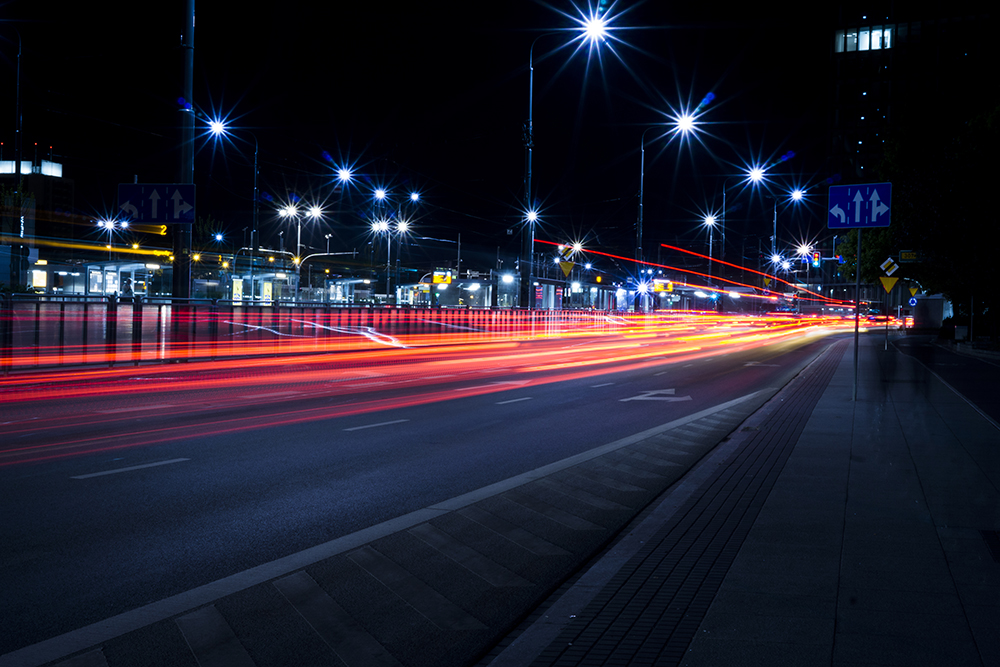
\includegraphics[height=\paperheight]{bg2.jpeg}
  }%
}


\begin{document}


%TITLEPAGE
%CHANGE TITLE PAGE
\renewcommand\maketitle{\newpage
\BgThispage
\newgeometry{margin = 0in}

\includegraphics[width=2.00in]{transpire.png}
\setlength{\fboxsep}{0pt}
\hfill \makebox[3.22in][r]{\shortstack[r]{\vspace{2.75in}}}%
\vspace{-0.25pt}
\setlength{\fboxsep}{10pt}
\setlength{\fboxrule}{0pt}
\colorbox{orangeBack}{\makebox[8in][r]{\hfill \shortstack[r]{\fontsize{36}{36}\sffamily\color{white} Strategic Management Plan\\%
\fontsize{20}{20}\sffamily\color{white} Reducing Travel Time and Traffic Congestion in Auckland}}}%
\setlength{\fboxsep}{0pt}
\vspace{-8.5pt}
\hfill \hspace{.21in} \parbox{2.97in}{\vspace{4.5in} \color{white} \textbf{\theauthor \\ \\   \thedate \vspace{2.3in} \vfill}}%
\let\Title\thetitle
\restoregeometry}
\begin{titlepage}
\maketitle
\end{titlepage}


%COVER SHEET - INCLUDE
\newlength{\normvoffset}
\setlength{\normvoffset}{\voffset}
\newlength{\normhoffset}
\setlength{\normhoffset}{\hoffset}
\setlength{\voffset}{0cm}
\setlength{\hoffset}{0cm}
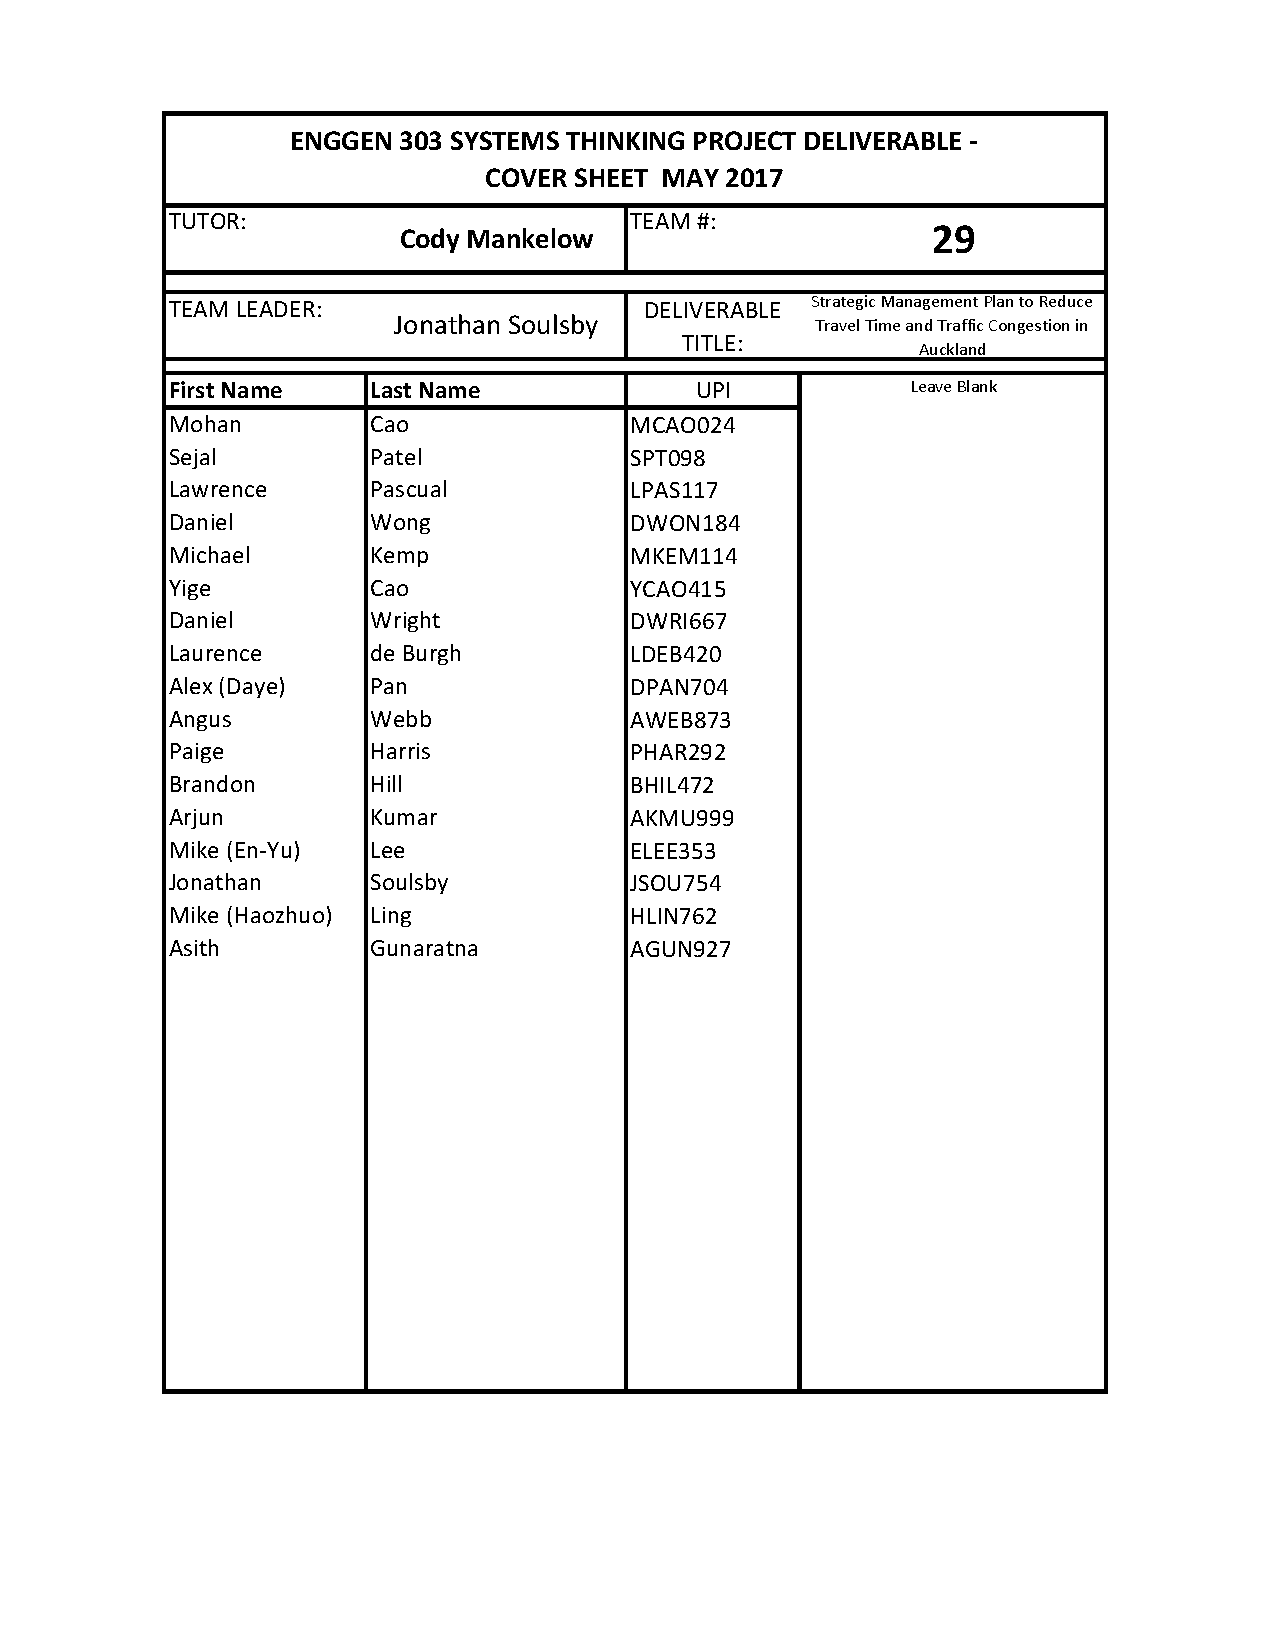
\includepdf[pages=-]{SYSTEMS_COVER_SHEET_FINAL.pdf}
\setlength{\voffset}{\normvoffset}
\setlength{\hoffset}{\normhoffset}
\newpage


%HEADER - Team name
\lfoot{\theauthor}
%FOOTER - Title
\lhead{Strategic Management Plan to Reduce Travel Time and Traffic Congestion in Auckland}
%FOOTER - Enables right foot page numbers
\rfoot{\thepage}
%CONTENTS - Adds Executive summary to the table of contents
\addcontentsline{toc}{section}{Executive summary}
\section*{Executive summary}
Transpire Consulting has been tasked by a New Zealand Government organised working group to develop a strategic management plan that will reduce travel time and traffic congestion in Auckland during peak hours. They have suggested looking into Smart Traffic Lights as a potential resolution, but have also requested a long-term solution to accommodate Auckland's growing population. The proposed Smart Traffic Management System targets the three root causes of congestion in Auckland: excessive traffic volumes, underdeveloped transport infrastructure and poor driver behaviour.\\

The Smart Traffic Management System consists of three parallel components: the introduction of a toll for drivers entering the Central Business District (CBD), the development of a transport hub located in Mount Roskill which will support increased bus routes, and the implementation of a Smart Traffic Control network. The solution is projected to be valid for a minimum of 20 years. \\

The toll implementation and transport hub are to be conducted concurrently to ensure a similar completion time of two years. Commuters that would normally take vehicles into the CBD will be incentivised to use the upgraded public transport system. In order to further streamline traffic flow, a Smart Traffic Control network will also be developed in the following years. This network of smart traffic lights and optimisation algorithms will gather data on vehicle positions and numbers. This enables the coordination of intersections and other traffic signals to improve traffic flow both within the CBD and the surrounding suburbs. The implementation of this solution has been carefully considered in order to keep disruption to the city to a minimum while ensuring the project is completed as fast as possible. At the 6 year mark, the Smart Traffic Control network will be fully functional and operable.\\

This proposed solution consists of more than one component as our detailed analysis of Smart Traffic lights ruled them out as an independently viable solution. It is expected that the Smart Traffic Management system will significantly reduce travel times during both peak hours and down times. Along with the economic boost as a result of increased productivity, the toll revenue is able to be funnelled into future projects. With fewer cars on Auckland's roads (since more of the population takes public transport), the environmental benefits will support New Zealand's international clean, green image. Exploration into available resources and funding shows that this proposal is economically viable and within the realm of current public spending budget allocations.The approximate total implementation cost of our proposed solution is \$143.2 million, excluding toll revenue.\\

The solution outlined in this report will relieve congestion in central Auckland during peak hours and is able to adapt to a growing city populous without the need to construct additional roads.
\newpage
%CONTENTS - Renames contents to Table of Contents
\renewcommand{\contentsname}{Table of Contents}
%FIGURES - Renames list of figures to Table of Figures
\renewcommand{\listfigurename}{Table of Figures}
%TABLES - Renames list of tables to Table of Tables
\renewcommand{\listtablename}{Table of Tables}
\fancypagestyle{plain}{
  \fancyhf{}
    \lfoot{\theauthor}
    \lhead{Strategic Management Plan to Reduce Travel Time and Traffic Congestion in Auckland}
    \rfoot{\thepage}
    \renewcommand{\headrulewidth}{5pt}
    \renewcommand{\headrule}{\hbox to\headwidth{%
      \color{orangeBack}\leaders\hrule height \headrulewidth\hfill}}
    \renewcommand{\footrulewidth}{5pt}
    \renewcommand{\footrule}{\hbox to\headwidth{%
      \color{orangeBack}\leaders\hrule height \footrulewidth\hfill}}
}
\tableofcontents
\fancypagestyle{plain}{
  \fancyhf{}
    \lfoot{\theauthor}
    \lhead{Strategic Management Plan to Reduce Travel Time and Traffic Congestion in Auckland}
    \rfoot{\thepage}
    \renewcommand{\headrulewidth}{5pt}
    \renewcommand{\headrule}{\hbox to\headwidth{%
      \color{orangeBack}\leaders\hrule height \headrulewidth\hfill}}
    \renewcommand{\footrulewidth}{5pt}
    \renewcommand{\footrule}{\hbox to\headwidth{%
      \color{orangeBack}\leaders\hrule height \footrulewidth\hfill}}
}
%CONTENTS - Generates
\listoffigures
%TABLES - Generates
\listoftables
\fancypagestyle{plain}{
  \fancyhf{}
    \lfoot{\theauthor}
    \lhead{Strategic Management Plan to Reduce Travel Time and Traffic Congestion in Auckland}
    \rfoot{\thepage}
    \renewcommand{\headrulewidth}{5pt}
    \renewcommand{\headrule}{\hbox to\headwidth{%
      \color{orangeBack}\leaders\hrule height \headrulewidth\hfill}}
    \renewcommand{\footrulewidth}{5pt}
    \renewcommand{\footrule}{\hbox to\headwidth{%
      \color{orangeBack}\leaders\hrule height \footrulewidth\hfill}}
}
\newpage
%FOOTER - Start at 1 with first section
\pagenumbering{arabic} 
%HEADER - Section
\rhead{}

\section{Introduction}
Rush hour travel is a notoriously slow and arduous process for a large portion of Auckland's commuters. Poor public transport systems and ageing motorway networks have resulted in lengthy and prolonged intra-city travel being expected for the wide majority of Auckland's population. In conjunction, Auckland's geography limits the land resources for new future-proofing projects and so requires the city to keep up with demand by constantly upgrading existing infrastructure. Auckland's geography again increases this challenge due to the narrow nature of the Isthmus zone and the narrow accessibility of the Central Building District's transport routes. These routes must meet demand in order for Auckland to function as a modern capital city, or face crippling travel times for trade and commuters in New Zealand's 'City of Sails'.\\

Congestion has many negative side effects that hinder a progressive city's function and growth. As well as extended travel times and inability to judge journey time requirements, the likelihood of accidents increases, emergency services are hindered, and large quantities of fuel are burnt for no return, offsetting New Zealand's 'green' image. From an analysis carried out in 2013, the estimated cost per year of vehicle congestion to Auckland city was \$1.25 billion compared to free-flow conditions, and \$250 million per year compared with the network operating at capacity \citep{wallis15}.\\

With an ever-changing, expansive and diverse city such as Auckland; efficient transportation and travel solutions are becoming harder and harder to develop, which is only expected to increase in difficulty as Auckland's population grows. Therefore the optimisation and streamlining of existing infrastructure has been prioritised to eliminate the construction of new roads, as desired by our client.\\

Considering Auckland's current day transportation, Transpire Consulting has been requested to identify and implement a long-term strategic management plan that will reduce travel time and traffic congestion in New Zealand's most populous city.

\subsection{Present Situation}
Based on NZTA statistics in 2016, the current allocation of government spending for the Auckland region alone on maintaining, building, and managing roads consumes up to \$1.5 billion out of New Zealand's approximate \$4 billion budget \citation{nzta16}. In fact, passenger transport spending was estimated at \$400 million - vehicle purchasing and maintenance inclusive. Despite this, poor travel times and sub-par traffic flow are still present problems still seemingly unaddressed in the current day; and have failed to remove Auckland's reputation for poor commuter travel. This is evident as a growing problem, with road users experiencing a 10\% increase in travel time delays to 40 - 47 seconds/km over 2014-2015 \citep{transport16}.

\subsection{Scope}
Transpire Consulting has considered possible solutions within a maximum time frame of 10 years, that must support and accommodate the growth of Auckland City. The geographic scope is limited to the Isthmus zone and City, defined by Auckland Transport (AT), as this most efficiently covers the most congestion hot spots. (\cref{fig:auckgeozones})(\cref{fig:lchs})

\begin{figure}
\centering
\begin{minipage}{.5\textwidth}
  \centering
  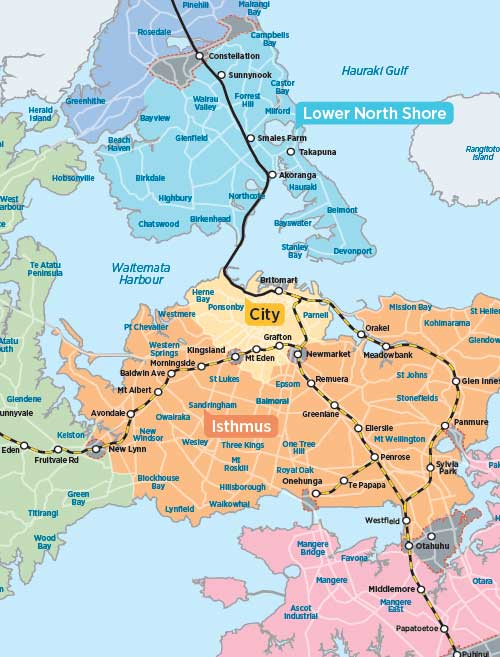
\includegraphics[width=0.8\linewidth]{Auckland_Geographical_Zones.png}
  \captionof{figure}{Auckland Geographical Zones}
  \label{fig:auckgeozones}
\end{minipage}%
\begin{minipage}{.5\textwidth}
  \centering
  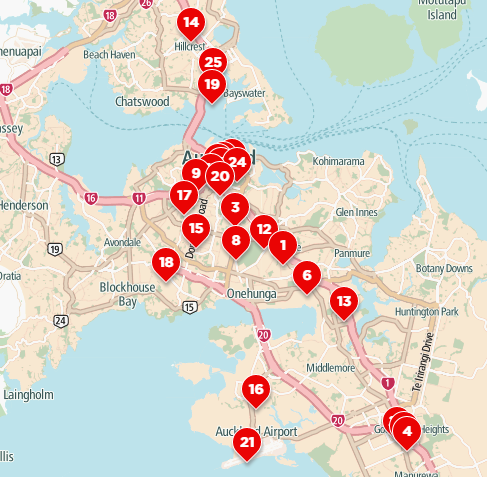
\includegraphics[width=0.8\linewidth]{Localised_Congestion_Hot-Spots.png}
  \captionof{figure}{Localised Congestion Hot-Spots}
  \label{fig:lchs}
\end{minipage}
\end{figure}



For the sake of analysis; peak hours are defined to lie within 6:00am-10:00am and 3:00pm-7:00pm. Any proposed solution may make road alterations to existing infrastructure including roundabouts, lanes and intersections. A minimum safety assumption is ensured that the solution matches or exceeds current safety factors.\\

The solution must use existing road infrastructure (i.e. contain no construction of new roads) and it should be noted that projections made in this report are estimates, and should be regarded as such.
\subsection{Problems}
Prefatory research and information identified the following problems that the Smart Traffic Management System needs to addressed.
\subsubsection*{Number of Cars on the Road}
Traffic congestion occurs as road use increases, and is characterized by slower speeds, longer trip times, and increased vehicular queueing. This is due to inefficient car usage in terms of lack of car-pooling, rush hour travel and in general: too many vehicles on the road at any given time. The intended solution for this problem is to increase number of passengers per vehicle whilst simultaneously decreasing private vehicle usage and encouraging alternative travel options in the form of public transport.
\subsubsection*{Infrastructure}
This category encompasses the solutions that the government incorporated, which in turn failed to fully meet demand. These include poor public transport, implementation of motorway on-ramps, corridors that run into the CBD, and unsophisticated traffic management systems, which add up to \$1.1 billion of government funding in 2016.
\citep{nzta16}
\subsubsection*{Driver Behaviour}
Sudden braking, resulting in braking repercussions  that ripple down the road, and road occupying drivers searching for car parks on main roads are just a few of many driver-responsible factors exacerbating Auckland traffic problems. However, the effect of these factors are hard to control and even harder to measure.
\subsection{Assumptions}
Throughout our report we will be making several assumptions. If our proposal is carried forward, these assumptions will have to be addressed, and are listed as follows:
\begin{itemize}
\item Project costs will come from current Government funding based on previous years' figures and supplemented through revenue generated by the Smart Traffic Management System's toll booths.
\item Data from Government Corporations and NZTA are accurate enough to extrapolate future costs.
\item Auckland Population growth rate continues to grow at a constant rate of 1.5\% over the estimated project operation time. \citep{stats17}
\item Catastrophic and disastrous out of line events do not occur between now and 2024.
\item There will be no vastly superior ground-breaking technology that is developed which voids the Smart Traffic Management System over the course of its implementation.
\end{itemize}


\section{Stakeholder analysis}
Traffic congestion is a voluminous issue that is common in developed urban regions such as Auckland City. These areas tend to be the commercial hubs of a nation, compacted together with a large proportion of the population. Therefore, it is indispensable to consider parties which could be influenced both directly and indirectly by the introduction of the Smart Traffic Management System. A stakeholder analysis is used to analyse the qualitative information of an independent party (or person) whose interest, requirements and influence should be taken into account when planning such a project. These factors determine how important they are with respect to the project and are listed below in that order.

\begin{enumerate}[label=\textbf{\arabic*}),leftmargin=0in]
\item \textbf{New Zealand Cabinet}
\end{enumerate}

The New Zealand Cabinet are the main clients associated with this project and hence the primary stakeholder. They will oversee and make the final decision on a solution to control the Auckland transport system as well as managing the reallocation of funding in the public spending budget.

Their intention is to reduce traffic congestion in Auckland and have suggested to implement a smart traffic light system as a solution. They are interested in other alternatives, permitting that there is sufficient funding after reallocation within the public spending budget. The NZ Cabinet requires the project to stay within the public spending budget while proposing a solution to improve traffic congestion in Auckland City. As they will make the final decision regarding the project and funding, both their interest and influence is high.

\begin{enumerate}[label=\textbf{\arabic*}),leftmargin=0in,resume]
\item \textbf{Auckland Road Users}
\end{enumerate}

The main goal of this project is to improve commute time for the population of Auckland that utilise roads and other relevant infrastructure for their travels. Examples include, but are not limited to cyclists, public transport users, pedestrians and private motorists. 

As a stakeholder, Auckland road users hold a high degree of importance, they are the majority of victims suffering from poor travel times as a result of traffic congestion. Their primary interest is that the proposed solution will reduce traffic congestion without imposing a significant inconvenience to their travels.

\begin{enumerate}[label=\textbf{\arabic*}),leftmargin=0in,resume]
\item \textbf{Auckland Transport (AT)}
\end{enumerate}

AT is responsible for the transport infrastructure, public transport, as well as the construction and maintenance of roads and traffic lights in Auckland \citep{ATND_2}, on behalf of the Auckland City Council. Currently, the Sydney Coordinated Adaptive Traffic System (SCAT) cannot fully satisfy transport demands. Their high level of influence is shown through their coordination with other stakeholders, for example ensuring minimal disruption to the current system and Auckland road users. 

AT's main interests incorporates long and short-term work plans in conjunction with network performance and safety, strategic outcomes, and network capacity. Their ultimate goal is to ensure safe and efficient commutes of Auckland residents to their destination. They require a high standard of reliability, safety and economical benefits from a new system.


\begin{enumerate}[label=\textbf{\arabic*}),leftmargin=0in,resume]
\item \textbf{New Zealand Treasury}
\end{enumerate}

The New Zealand Treasury hold responsibility for providing advice and assistance to the government and its departments regarding economic growth and financial planning. They assist with planning government finances from different sectors, of note, the transport sector included. 

The New Zealand Treasury will also be highly influential in coordinating the project with regards to assisting the New Zealand Cabinet in reallocating the budget of any solution proposed by Transpire Consulting. By working with other transport agencies including AT, NZTA and the Ministry of Transport, they address concerns regarding policies and funding with respect to this project \citep{treasury16_2}.

\begin{enumerate}[label=\textbf{\arabic*}),leftmargin=0in,resume]
\item \textbf{New Zealand Transport Agency (NZTA)}
\end{enumerate}

The NZTA is partnered with the Ministry of Transport to coordinate with other influential stakeholders \citep{nztaND} to ensure a safe and functional transportation system, including the allocation of funding to land transportation projects. 

The NZTA's interests include the network performance and safety outcomes, network standards, subsidy funding levels, as well as providing economical value to Auckland City. As they hold a key focus in the safety of parties involved with travel related projects, the proposed solution must comply with relevant safety regulations and standards.

\begin{enumerate}[label=\textbf{\arabic*}),leftmargin=0in,resume]
\item \textbf{Ministry of Transport}
\end{enumerate}

The Ministry of Transport is the New Zealand Government's principal transport advisor. Through their advice, they aim to improve the performance of New Zealand transport systems and work with local government authorities to carry out land transport plans that in turn guide the decision making of any related transport project \citep{mot17}. In the case of this project they will be working alongside Auckland Transport.

The Ministry of Transport will be managing the funding allocated by the government towards the project as well as giving advice to Auckland Transport on the viability of any proposed solution; especially in the long term \citep{mot17_2}. Through this project they wish to improve Auckland's existing transport options, reducing travel time and traffic congestion, especially during peak travel hours.


\begin{enumerate}[label=\textbf{\arabic*}),leftmargin=0in,resume]
\item \textbf{Taxpayers}
\end{enumerate}

Taxpayers are individuals and businesses who pay a mandatory fee to the government for national funding. Both Auckland taxpayers and non-Auckland taxpayers will have an influence to some degree with this project.\\

\textbf{Auckland Taxpayers:} Collectively, they will have a high interest and a moderate influence (financially) towards this project. This is because they are directly impacted by traffic congestions and look forward to having this issue rectified.\\

\textbf{NZ Taxpayers excluding Auckland:} They will influence this project to some extent financially; however, they will not display much direct interest in this project as local traffic congestion and travel time will not be affected in their regions. However, some will have resistive opinions in regards to the reallocation of funds from their regional budget. Hence their primary concern is the movement of taxpayer funding out of local projects directly affecting them, and into any proposed solution by Transpire Consulting.


\begin{enumerate}[label=\textbf{\arabic*}),leftmargin=0in,resume]
\item \textbf{Industry and Service Providers}
\end{enumerate}

Industry and Service Providers include freight, delivery services, and other commercial companies that require the use of land transportation. Reducing congestion will reduce the company's cost in both travel time and fuel cost, promoting growth and profitability. They will be interested in the transportation network performance (improved traffic flow and public transport), scheduling, ticketing, information systems, and service subsidies.

\begin{figure}
\centering
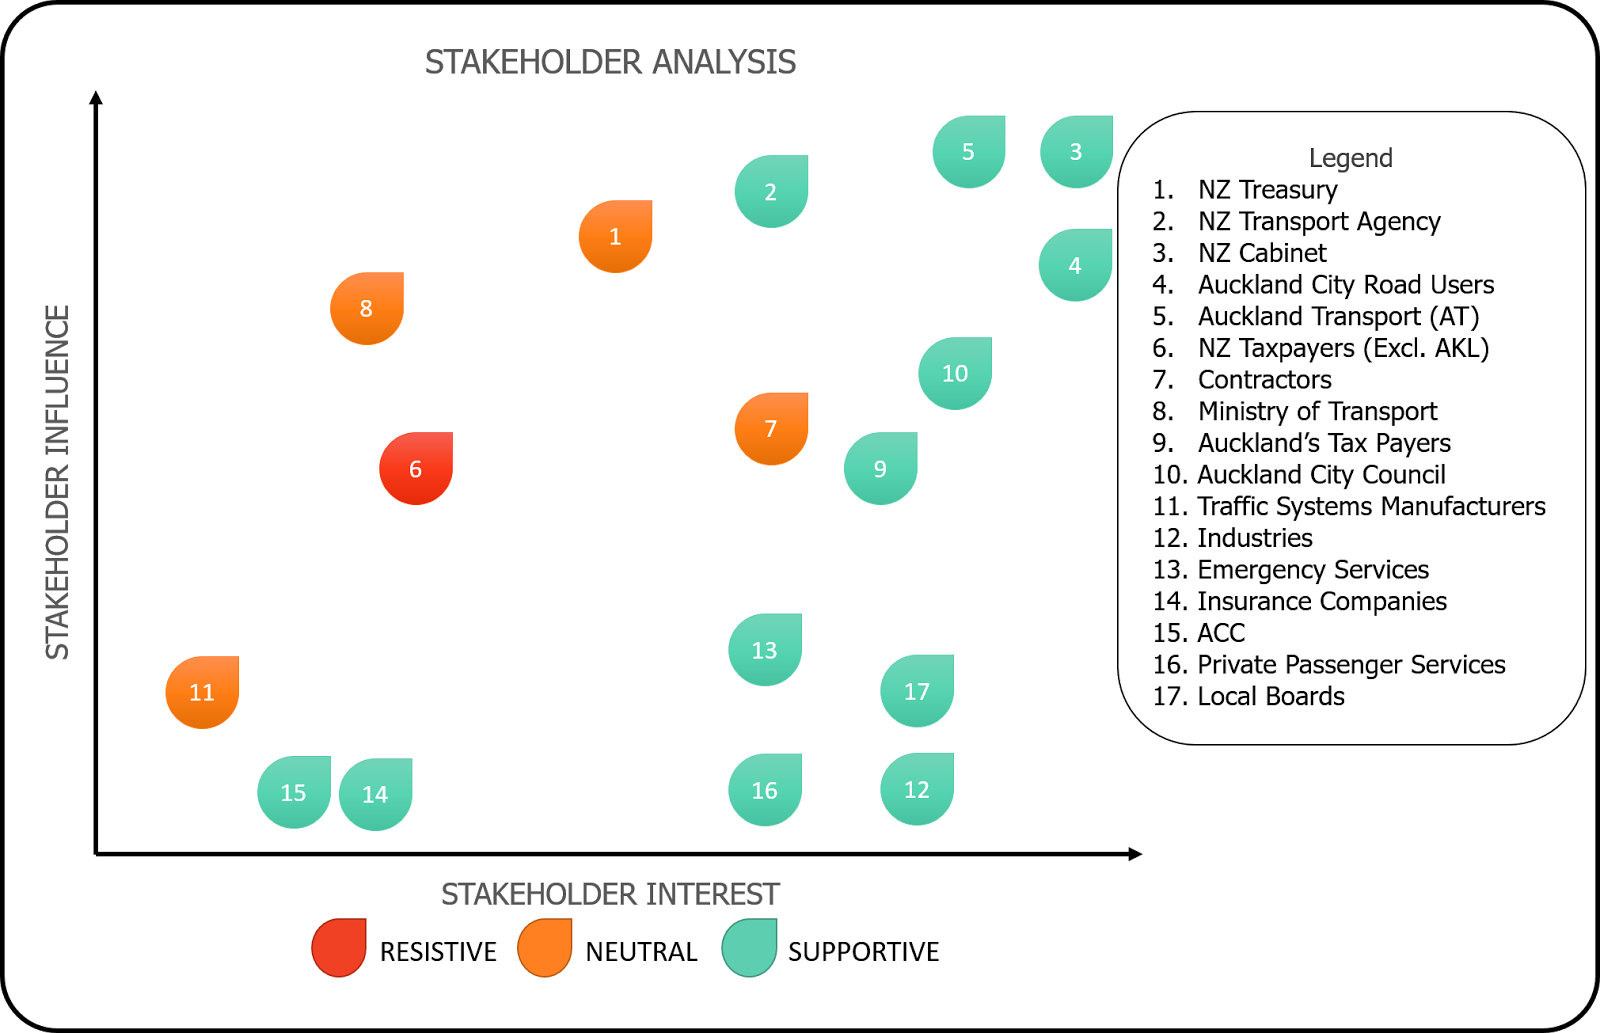
\includegraphics[width=\textwidth]{Picture5.png}
\caption{Stakeholder chart of major and minor stakeholders with outcome effects}
\label{fig:stakeholder}
\end{figure}

It can be seen in  (\cref{fig:stakeholder}) that a large majority of stakeholders, especially major influential stakeholders, arie supportive and interested as they would benefit from this project. There is a single resistive stakeholder, ``NZ Taxpayer excluding Auckland (Excl. AKL)'', because it does not benefit them directly.
\newpage


\section{Requirements}
Having thoroughly considered the requirements of all the primary stakeholders, a list of best fit requirements have been compiled. These are to be used in the implementations that will best meet the long term goals of a strategic management plan aiming to reduce travel times and traffic congestion.

\subsection{Economically Viable}
According to New Zealand's 2016 budget, \$2.1 billion has been allocated towards public infrastructure \citep{gov2016}. The primary inconsistency within stakeholders lies between local and other regional taxpayers. Reallocation of taxpayer funding to localised areas will indefinitely conflict regions in which funding is cut from. To avoid conflict, any proposed solution must aim to minimise dependency on externally allocated taxpayer funding.


\subsection{Decreases Traffic Congestion}
This is an essential requirement as major stakeholders such as Auckland Transport, NZTA, and Auckland road users share a consistent and common goal; reducing and improving travel times. Ultimately, proof of a successfully developed and implemented proposed solution will result in a reduction in traffic congestion and benefit all road users.


\subsection{Future Proof and Long Term}
As the scope of the project is long term, decisions made need to be considered with the mindset that a large scale project of this nature is unlikely to be completed instantaneously. Implementations should retain a degree of flexibility to account for unforeseen changes in the near future.

\subsection{Avoids Construction of New Roads}
The main stakeholder, the NZ Cabinet, has specified that construction of new roadways are not to be undertaken. However, this could lead to difficulties in the future for Auckland motorists, especially regular motorway users, as the current road system does not take into account Auckland's growing population\citep{herald17}. However, with focus on other alternative options, this requirement can be worked around.

\subsection{Environmentally Sustainable}
With growing concerns about the global climate and the spotlight on sustainability, it is a requirement from all stakeholders to keep greenhouse gas emissions to a minimum during the construction and use of any proposed solution. This will be consistent with all stakeholders in the long term as decreasing greenhouse gas emission will benefit New Zealand's `green' image, and the living standards of New Zealand's population as a whole.

\subsection{Safety}
The solution needs to meet or surpass the safety ratings of the current traffic management systems. The safety of Auckland Residents on the road is of utmost importance. This means the fatality/injury rate on Auckland roads can not increase, and ideally will decrease. Additionally, the solution selected should be capable of handling large fluxes in the composition and density of traffic flow, as well as withstanding Auckland's temperamental weather pattern. Auckland Council and Auckland Transport should be able to rely on the proposed solution to manage the traffic of Auckland City without causing any immediate impact to the system users. In particular, the new system must comply with relevant New Zealand and global standards enforced by the Ministry of Transport. Any safety issues should be systematically recorded, documented and reviewed.

\subsection{Resource Efficient}
The implementation of the project should utilise all resources that are available. This includes - but is not limited to - money, time, equipment, manpower and land.  Management of resource efficiency will consequently result in increased cost-savings. Hence, all stakeholders will be consistent together with this requirement as a waste of resources would not be economically viable due to constraints in the budget.

\subsection{Publicly Accepted}
The project must earn public acceptance since they will engage and utilise the project outcome thereafter. If the project is not used by the Auckland public, the key stakeholders will be unsatisfied due to the wasting of resources (time, funds, labour and materials). Hence, they are in a consensus that this is is an important requirement. To achieve public acceptance, it is required that appropriate testing and documentation is conducted.

\subsection{Transparent}
Project transparency improves the public accountability of the organisations involved and increases public understanding of the project. In addition, it enhances the communication between stakeholders and productivity. Stakeholders involved should easily access and work with project information at any point in time especially if any difficulties or constraints are encountered.
\newpage


\section{Possible Solutions}
Extensive research was done by Transpire Consulting investigating possible solutions that could be implemented as part of a long-term strategy to reduce travel time and traffic congestion in Auckland, with the root causes being categorised into three main factors: the sheer volume of traffic on the road, current transport infrastructure and poor driver behaviour.
 
\subsection{Banning Cars from the Central Business District and Introducing a Shuttle Service }
Currently the majority of congestion is concentrated in the CBD. 111,000 employees are located there and universities and other educators account for at least 60,000 students \citep{MattL17}.. The removal of cars allows for a more streamlined construction of the existing plans for the Light Rail which would correspondingly increase in demand. This option also creates a safer city centre, encourages inner-city economic development and substantially reduces visual, noise and environmental pollution. Should commuters still opt for private transport, they musts find parking outside the CBD and either make use of public transport or walk/cycle into the city.
\\In conjunction with the removal of cars in the CBD, a licensed shuttle service can be implemented to streamline travel around the city, with a simple tag on/off implementation. This option is also attached with a high level of flexibility as shuttles are not permanent structures and can be discontinued should the Light Rail be completed and deem the service redundant in the future.

\subsection{Introducing an Electronic Toll for Cars Entering the CBD}
Tolls and road charges are an effective method to discourage road use. These toll roads use electronic chips inside cars to charge users travelling into the CBD. The benefit of the electronic toll is that it does not require the cars to stop or even slow down, allowing them to continue travel with zero interference. Public transport and heavy commercial vehicles would be exempt from these charges, encouraging commuters to a cheaper, more environmentally friendly alternative and allowing industrial access to the ports respectively. Drawing inspiration from existing sources; London implemented a similar system, adding a charge to certain congested areas, which resulted in a drop of car usage of 20\% and the biggest growth of the bus system since the 1940's. \citep{joepeach11}
\\The issue with this solution revolves around setting up this scheme. Implementing the toll booths and installing electronic chips in all cars would be very costly, however decreasing the amount of traffic on the roads, easing congestion and providing revenue to increase public transport infrastructure could offset this negative.
 
\subsection{Enforcing Carpooling}
Currently around Auckland there are various segments of T2 and T3 lanes on roads and motorway access. These lanes provide an exclusive lane for commuters who are carpooling. The idea is to encourage commuters to carpool as they can bypass the traffic. Carpooling provides benefits as they reduce the space taken per person commuting, i.e. if three people car pool, there are two less cars on the road taking up space. If more people carpool there will be less cars on the road thus reducing traffic congestion. An issue with this currently is that there are no coherent stretches of road with transit lanes, they are in small segments. If there were a main road with a transit lane stretching across its entirety, there would be more benefit and incentive to use it. Currently users have to merge in and out of transit lanes which is inefficient and causes further slowdown from merging.
 
\subsection{Smart Traffic Control Network}
Traffic lights throughout centres currently use plate sensors which receive signals when a vehicle enters the intersection \citep{ATND}. Current sensors cannot detect the type, number or the speed at which vehicles pass through the intersection. Smart traffic lights propose the use of real time data, altering the signal phasing as required with the use of cloud-based data from wirelessly connected, in-ground and micro radar sensors \citep{verizon16}. With 24 hour smart traffic lights continually monitoring and updating the user on how well intersections and roads are performing, data collection allows continual optimisation of phasing to shift and adapt as road behaviour changes.
\\Potential additions to provide further input data on congestion and vehicle statistics include increasing the number of cameras on main traffic lights to provide more accurate data. This data would be fed to a neural net or algorithm to calculate an output for an optimal solution for traffic phasing and speed. This data would be relayed to users via variable speed signs or a commuter application, as detailed below.

\subsubsection{Introducing Variable Speed Limit Signs (VSLS)}
Currently, approximately 56 percent of students aged 5-12 in Auckland are driven to school, according to a 2013 Ministry of Transport Household Travel Survey \citep{mot14}. The morning school run accounts for roughly six percent of overall traffic volume \citep{mot09} , however the timing and location of school commuters makes it an important area of interest when tackling the issue of traffic congestion.

VSLS are seeing an increase in usage by councils worldwide to reduce and manage traffic congestion along busy road sections, schools and safety zones. These signs can be set to display a lower speed limit at certain times, such as at the start or end of the school day, or during school events, but display the standard speed limit during other times of the day. 40km/h variable speed limits in school zones have been operating successfully in New Zealand since they were first installed on a trial basis in Christchurch in January 2000 \citep{nzta11}.
\\Evaluations made from this trial found that locations most likely to benefit from a variable speed limit in a school zone, are those that meet the following conditions:  
\begin{itemize}
\item are on arterial routes or multi-lane roads or high speed environments.
\item have on-road, school-related activity at an obscured school frontage (i.e where the presence of the school is not immediately obvious to approaching traffic).
\end{itemize}
Building on this, VSLS can be adjusted according to road surface and weather condition, as well as irregular disturbances such as road accidents and maintenance work. By activating these signs along quieter roads connecting to congested arterial routes, the `slowing' ripple effect (caused by excessive braking due to a large change in speed) environment is minimised. With the advantage of being able to efficiently steady the flow of traffic along roads of significance such as Auckland's Southern and Western motorways, VSLS are the intelligent alternative to static speed restrictions and work to improve driver behaviour.
 
\subsubsection{Implementing an Integrated Commuter Application with Traffic Control Hardware}
It is possible to aid traffic control through the use of an application. Utilising the location services of application users increases the number of discretely tracked cars. Integrating this solution with smart traffic lights enables efficient control inputs to flow. Individual drivers can also be given instructions to change lane, detour, allow emergency vehicles to pass etc., as well as general instructions to improve traffic flow. As we are only looking to improve peak times, the application is targeted at commuters and can incentivise businesses to get staff on board (such as through a privately organised reward system), but also can be applied to benefit a motorway user at any time. This could also integrate with smart parking to direct to available parking if needed. Commuters are incentivised to use the app as it will direct them along paths that decrease their travel time or give them priority. As well as this, the large amount of data gathered from users enables optimising algorithms to be developed to control smart traffic lights.
 
\subsection{Fast Tracking Light Rail Development}
The current public transport options in Auckland are unreliable and slow. Trains are on time but people still prefer to drive for convenience and speed. Buses possess both problems although AT has recently introduced double deckers with greater capacity. The light rail is a possible solution to the current public transport infrastructure. Travelling along the centre of the road at high speed, its increased capacity and frequency attracts more commuter use \citep{AT16_2}. This decreases the number of cars on the road and substantially improves the current public transport options.

\subsection{Replacing Traffic Lights at Intersections with Roundabouts}
Roundabouts are not only safer in terms of having lower accidents rates than traffic lights but also have faster traffic flow. In fact, rates of injury are reduced by 75\%, an appealing statistic for stakeholders such as insurance companies and the ACC \citep{wsdtND}. When approaching roundabouts cars have to travel at lower speeds, there is no light to beat, as well as the fact that the design of roundabouts eliminates head on collisions. Roundabouts also increase traffic flow by eliminating waiting time for the green light at traffic lights. Drivers are required to give way, not stop. A study from Kansas University has shown that roundabouts have reduced travel times by 20\% \citep{russeletal2002}. Therefore, this significantly increases its feasibility on par with other solutions. Roundabouts are also cheaper to implement than traffic lights. They do not possess the hardware, maintenance and electrical infrastructure and accommodating maintenance and repair costs that traffic lights have. Also, in terms of reliability such as power outages, roundabouts are superior to traffic lights in maintaining continuous flow. However, this is not ideal for every intersection, as they are biased towards the direction of heavier traffic flow. In this situation, cars coming from other directions have less opportunity to merge. Also, cyclists are particularly at risk at roundabouts due to their lack of ability to accelerate quickly. 
 
\subsection{Staggering School and Business Times}
One of the factors causing rush hour congestion is the sheer volume of cars going onto the roads at the same time. This is caused by schools starting at 8:30am and finishing at 3pm as well as the typical commuter starting at 8am and finishing at 5pm. As most commuters start and finish their work at similar times, transportation to and from the city are synchronised and hence congestion and `rush hour' traffic occurs. A potential solution would be to stagger the start and finish times of schools and businesses. This results in a dissipation of cars previously travelling during rush hour hence reducing traffic congestion and travel times.

\subsection{Improving the Existing Bus System}
Despite the presence of available buses open for public transport around Auckland, many people prefer to take personal vehicles. This lack of appeal stems from the disorganisation and lack of resources in the current bus system. There are often too few buses, buses arriving late, not enough coming, or they do not have enough stops which results in people having to walk annoying distances to the nearest bus stop. Another aspect that makes current bus transport an undesirable alternative to private transport is that, more often than not, it is slower. Increasing the frequency of bus stops, developing new routes and increasing the number of buses operating, would encourage the use of public transport and decrease the number of cars on the road. 
 
\subsection{Moving the Port of Auckland to Tauranga}
Moving the Port of Auckland to a suitable location elsewhere (such as Tauranga) would decrease the amount of traffic flow due to freight. Trucks drive slower than cars and take up more road space, and the removal of their presence would help relieve congestion on Auckland roads. It would be an extremely expensive project, but also open up the possibility to develop the Auckland waterfront to be more suitable for cruise ships and other commercial endeavours.
 
\subsection{Transport Hubs}
The development of transport hubs (such as Britomart station) would help streamline the current transport network. Transport hubs allow for efficient transfers between public transport routes, incentivise public transport usage, give people better access to jobs, education and housing, as well as provide more choice about how to get around Auckland. As well as this, by injecting a source of efficient public transport options into an area previously starved of convenient and accessible train/bus services, commuters in the nearby vicinity are encouraged to drop driving into the city for cleaner travel options while also minimising traffic congestion. 

\newpage


\section{Best-fit Solution}
After considering a range of possible solutions, a MART analysis (see appendices) was used to evaluate each solution's individual performance in comparison to one another. This was conducted by outlining the main factors that affect the implementation of any project. To ensure that the MART analysis is performed fairly, each factor was weighted depending on its importance to the project development. For this particular case, the factors are:
\begin{itemize}
\item Influence on traffic flow
\item Environmental benefits
\item Social benefits and drawbacks
\item Economic benefits and drawbacks
\item Time to incorporate the project
\end{itemize}

It was decided that influence on traffic flow was the most important, followed by economic, time, social and environmental factors.

Due to circumstances such as lack of funding, the feasibility of some projects have become questionable in terms of outputting the best solution. This does not take away from their potential to reduce Auckland's transport problem and would be helpful to implement in future projects. However, it was the projects that positively influenced the traffic flow the most that were recognised to be the most effective solution. Out of the fifteen possible solutions ideas, the top four were investigated further by performing a cost benefit analysis (see appendices). These four solutions were analysed against a time period of 25 years in order to satisfy the project's long term requirement.The results of the CBA are shown in \cref{cbares}.

\begin{table}[H]
\centering
\begin{tabular}{|l|r|r|}
\hline
Solution                                            & Benefit/Cost Ratio & Time to implement \\ \hline
Smart Traffic Control Network                       & 4.8                & 5 Years           \\
Light Rail                                          & 0.55               & 11 Years          \\
Electronic Tolls                                    & 15                 & 2 Years           \\
Transport Hub similar to Britomart in Mount Roskill & 7.1                & 2 Years\\          
\hline
\end{tabular}
\caption{Cost-Benefit Analyses Results}
\label{cbares}
\end{table}

The CBA determined that introducing electronic tolls for private cars entering the CBD would be the most effective solution at reducing travel time and traffic congestion. With an implementation time of only 2 years, it has an immediate impact. However, introducing a toll with no alternative is simply taxation and needs to be implemented alongside alternatives in order to be socially acceptable. The other solutions that have passed the cost benefit analysis work well in conjunction with the toll as outlined below, with the best-fit solution addressing the issue of long travel times and traffic congestion from three sides:

\begin{enumerate}
\item A Smart Traffic Management network which optimises traffic flow on the road and reduces the effect of shock-wave traffic jams. This allows for a greater volume of traffic to move through the grid at speed.
\item A toll booth ring around the CBD. This discourages private drivers from entering the CBD. Traffic numbers are reduced and car-pooling is incentivised.
\item A new public transport bus hub, in Mount Roskill, and drastically increasing bus numbers make use of the reduced traffic density outcome in the CBD, allowing more efficient travel elsewhere.
\end{enumerate}

These 3 parallel components were chosen as they solve the three main factors which cause congestion.

\subsection{Smart Traffic Management Network:}
Input Streams
\begin{itemize}
\item Data from the application, includes vehicle type, velocity, destination, and approximate location.
\item Existing bus tracking system with similar data collection as the application.
\item Variable speed limit signs include camera sensor to measure bulk traffic velocity.
\item Intersection cameras integrated into smart traffic light system.
\end{itemize}
These data streams are processed to optimise routes depending on requirements and time of day; prioritising public transport or emergency services while improving average travel times for all users.\\\\
Output Streams
\begin{itemize}
\item The app opens a communication channel to the vehicle operators, notifying them of lane changes, exits, changes in route, dynamic speed limits, and incoming emergency vehicles.
\item Variable speed limit signs coupled with the application allow all users to be notified of real-time per-sector speed limit changes to reduce the effect of shock-wave ripple traffic jams; slowing the incoming traffic to allow the ripple to fade and then the bulk traffic can accelerate to highway speed again.
\end{itemize}

This system, extending the entire geographical scope, relieves congestion for most of the wider Isthmus area, but has little optimisation potential in the narrow and cramped CBD. This is where the other two methods assist in improvements.


\subsection{Toll Stations Into CBD and Improvements to Bus Transport Network}

A toll booth system charging traffic into the central business district scored highest in our cost to benefit analysis. However, a toll system must be implemented in conjunction with major improvement of public amenities in order for the change to be received well.
As the toll decreases popularity of personal vehicles entering the CBD, decreased bus fares and increased bus density makes efficient public transport more appealing, and so vehicle density will decrease. Allocated funds allow installation of 20 booths, of which 17 are immediately required to sufficiently cover inroads to the Auckland Central Business District. Observations that will be made include, public reaction and driver behaviour to tolling with respect to the final funded three booths, constructed if required.

In conjunction with the tolling project undertaken, a new bus hub will be constructed in Mt Roskill. Mt Roskill was selected for the hub location due to its distance from existing major public transport infrastructure while retaining a close proximity to the CBD. This is with the aim to facilitate an increased bus density in the Auckland Isthmus, feeding into the transport-hungry CBD as car movements are restricted by the tolling booths. Further into the project execution, the smart traffic network facilitates greater number of affordable buses with the existing flow, making public transport a faster, cheaper option. This will require a lowering of bus fares, which will be made up by the tolling revenue.
\newpage


\section{Systems Architecture}
\begin{figure}[H]
\centering
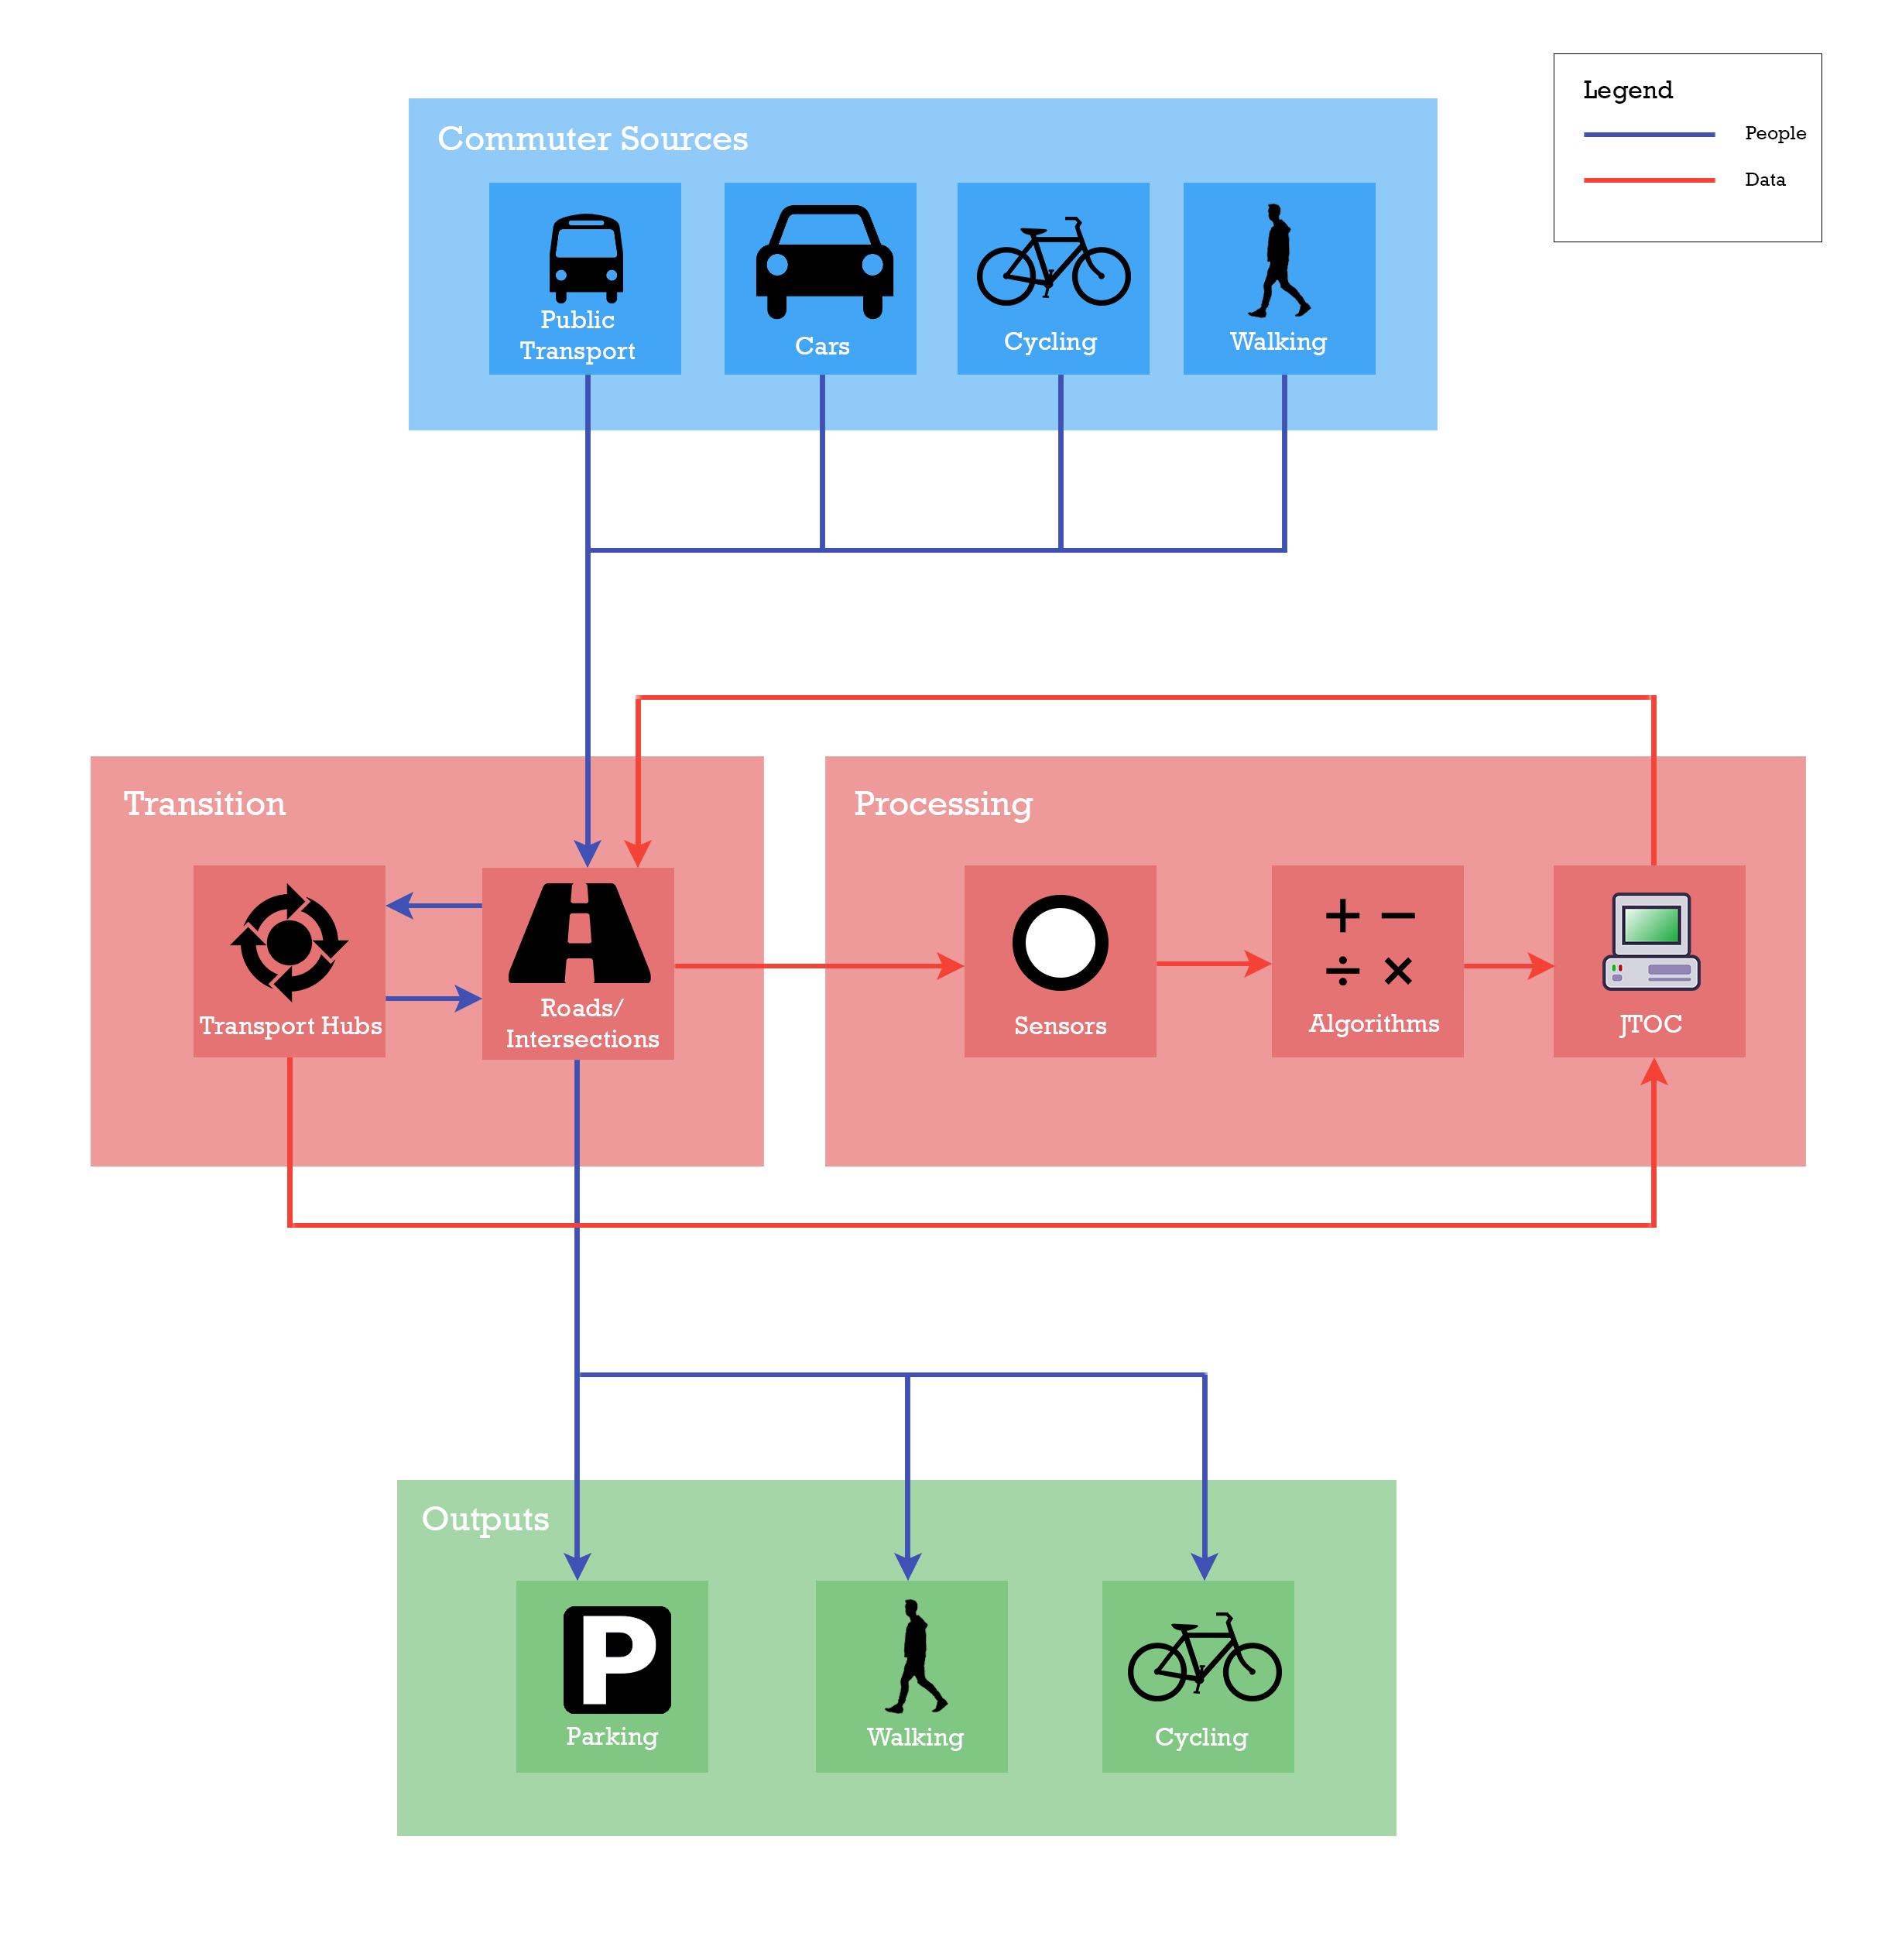
\includegraphics[width=\textwidth]{SystemsArchitectureCurrent.png}
\caption{Diagram of the current systems architecture}
\label{fig:sac}
\end{figure}
\newpage
\begin{figure}[H]
\centering
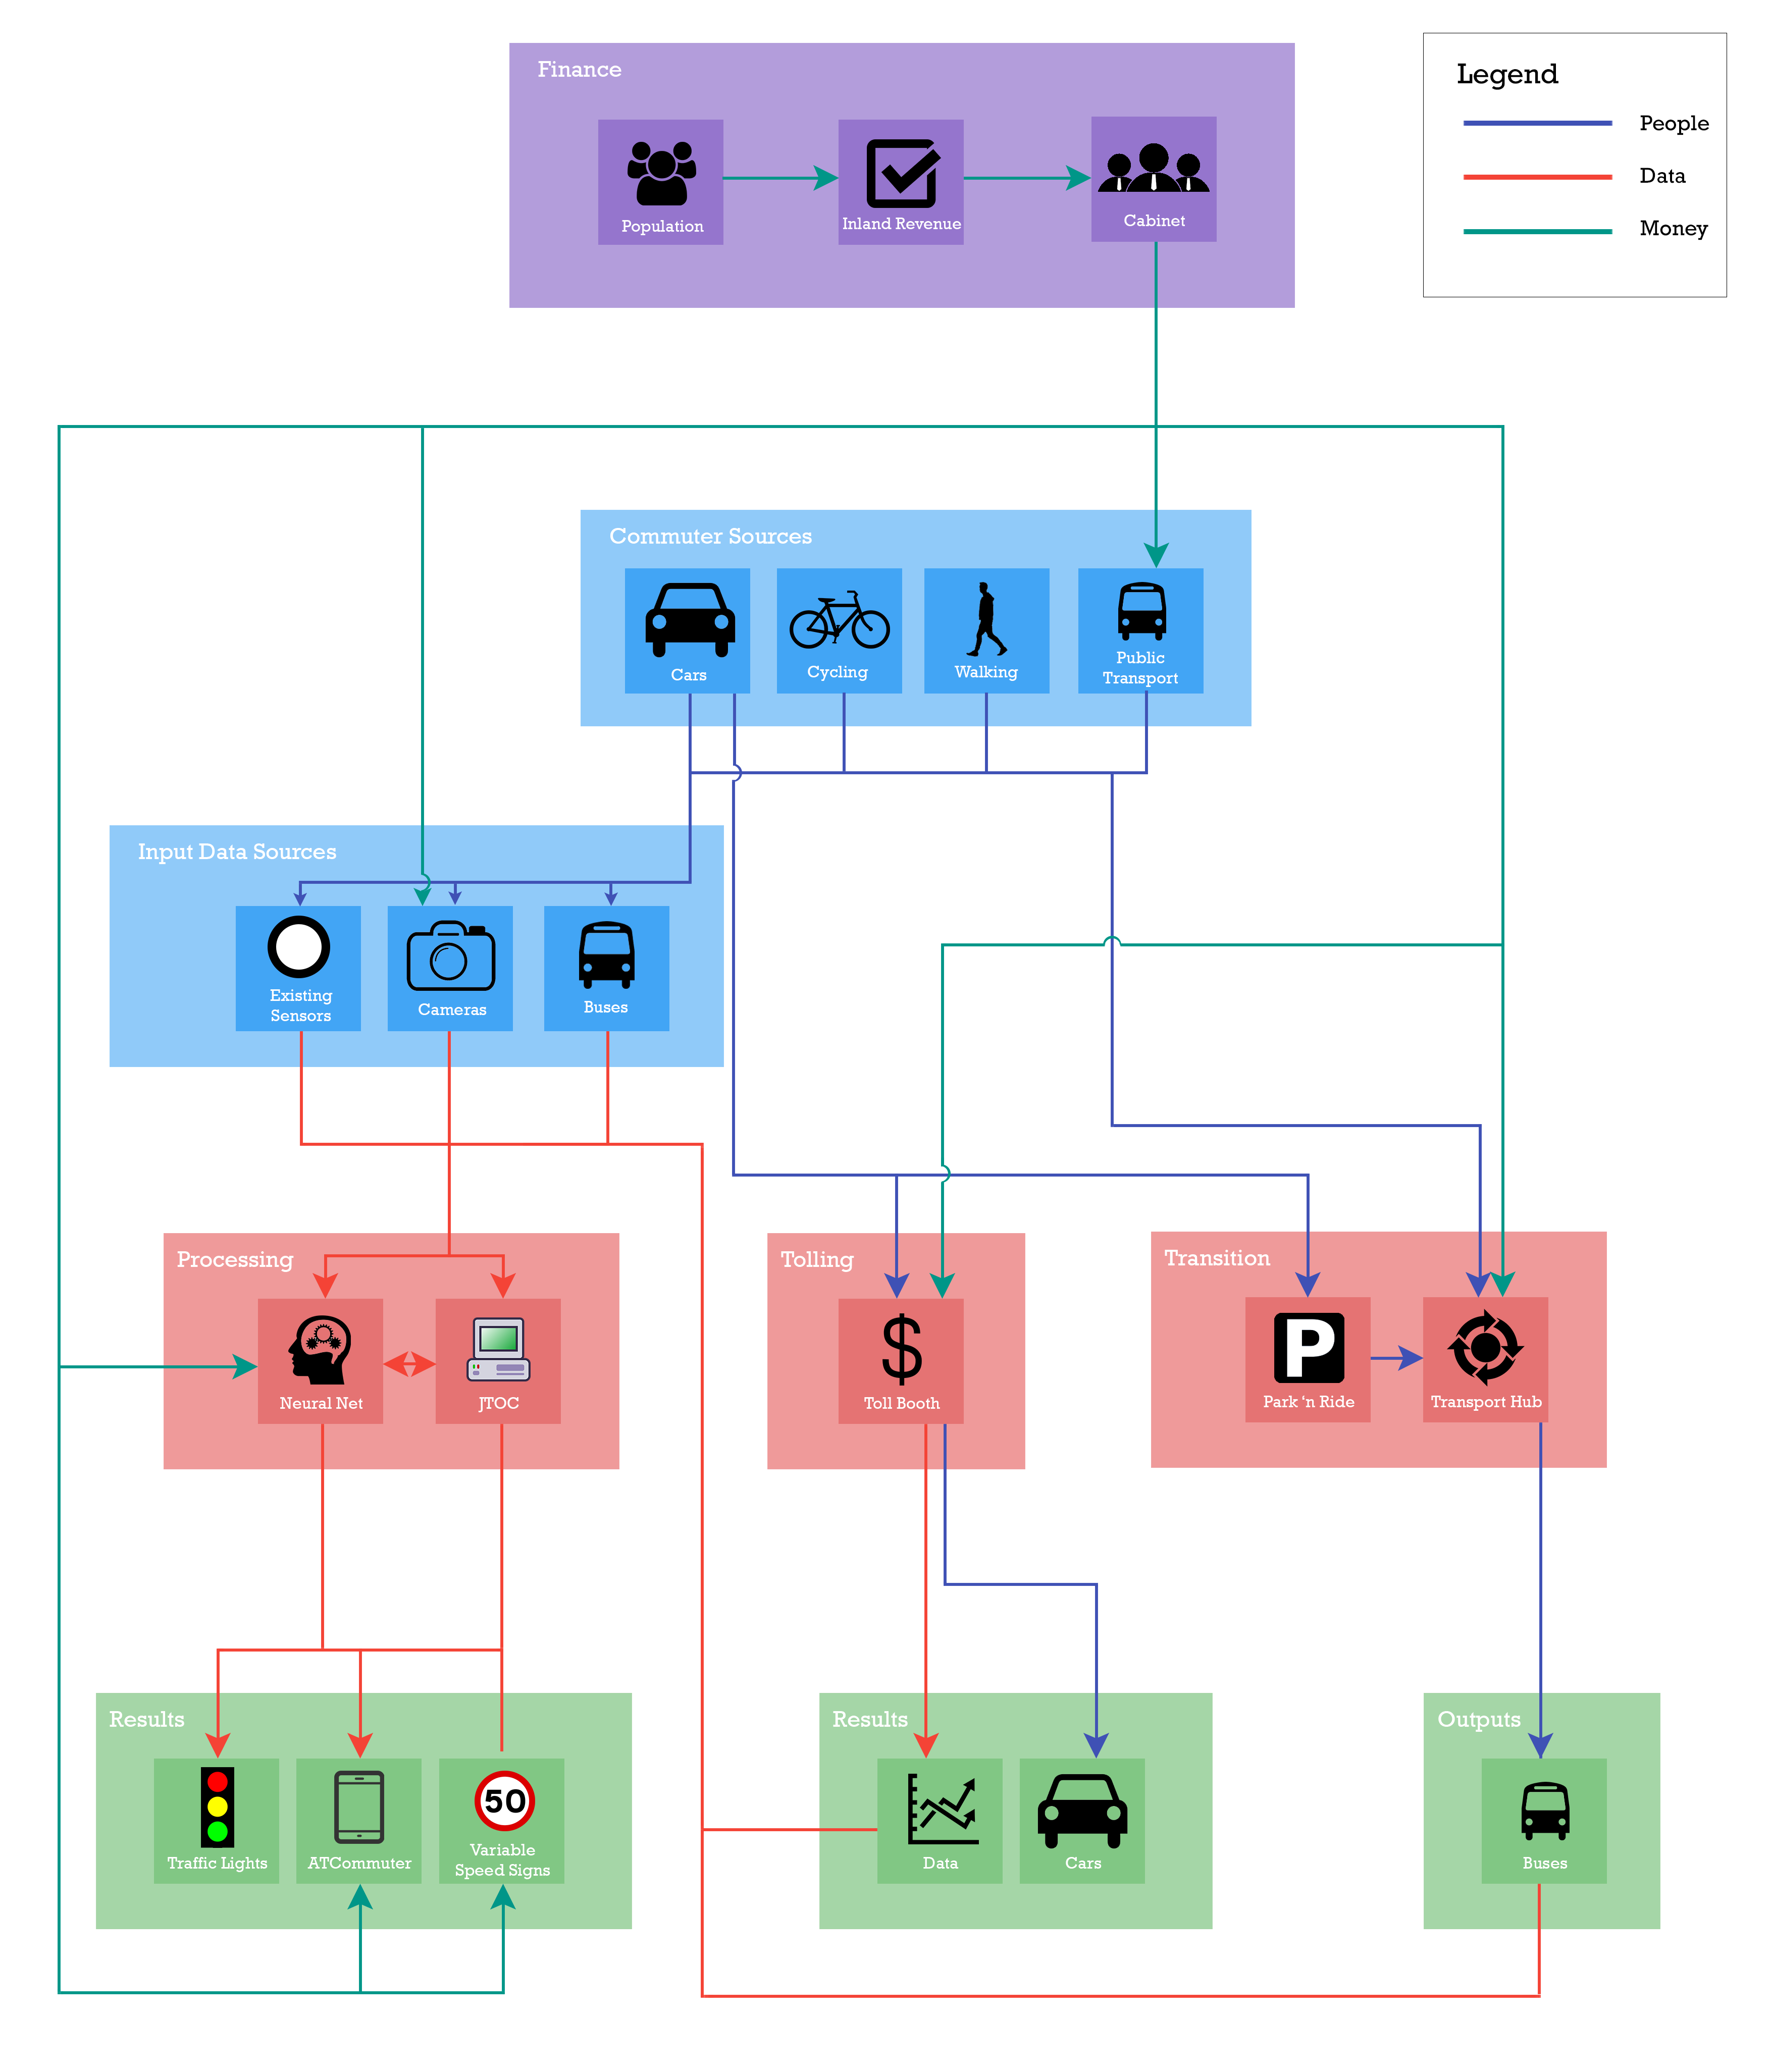
\includegraphics[width=\textwidth]{SystemsArchitectureNew.png}
\caption{Diagram of the proposed systems architecture}
\label{fig:san}
\end{figure}
\newpage


\section{Required resources}
\begin{table}[H]
		\centering
		\begin{tabular}{|p{6cm}|p{7cm}|}

			\textbf{ACTIVITY}                                                                 & \textbf{RESOURCES       }                                                                                                                                                                                                                                                                                                                                                                                                                                                       \\
			Approval of solution.                                                    & Lawyer services and legislative committee to advise if the solution is viable.                                                                                                                                                                                                                                                                                                                                                                                         \\
			Forecasting population growth and transport behaviour.                   & Personnel and funding for transport investigation.                                                                                                                                                                                                                                                                                                                                                                                                                     \\
			Integrating management team into the current Auckland transport network. & Additional personnel. Management plan.                                                                                                                                                                                                                                                                                                                                                                                                                                 \\
			Investigation and validation.                                            & Data collection and analysts to validate the best fit solution.                                                                                                                                                                                                                                                                                                                                                                                                        \\
			Plan and implement the transport development.                            & Lawyers/Surveyors. Execution of strategy.                                                                                                                                                                                                                                                                                                                                                                                                                              \\
			Local public announcement.                                               & Newspapers, media and social media.                                                                                                                                                                                                                                                                                                                                                                                                                                    \\
			Domestic transport behaviour incentives.                                 & Government incentive.Public transport. AT Hop Card availability.                                                                                                                                                                                                                                                                                                                                                                                                       \\
			Preparation for execution of plans.                                      & Funding to construct and implement `Smart Traffic Management' network. Consultancy on method of execution.                                                                                                                                                                                                                                                                                                                                                             \\
			Installation of `Smart Traffic Management' system.                       & \begin{tabular}[c]{@{}l@{}}Smart network development: \\      ATCommuter software development.\\      Variable speed sign acquisition and installation.\\      Smart traffic light acquisition and installation.\\ \\ Toll booth stations: \\      Material sourcing\\      Installation labour\\ \\ Transport development:\\      Material sourcing\\      Land sourcing\\      Labour and management of construction\\      Employees (bus drives etc).\end{tabular} \\
			Management of infrastructure                                             & Both the toll booths and the transport hubs would require personnel to maintain, run and manage them. Material would be required to fix and upgrade our equipment.                                                                                                                                                                                                                                                                                                     \\
			Management of funding                                                    & Ensure allocation of profit to the continual maintenance of infrastructure.Allocate remaining profit to future transport development plans.                                                                                                                                                                                                                                                                                                                            \\
			Management of future funding                                             & After the system has been implemented the government/Auckland council will manage funds and keep the system running.                                                                                                                                                                                                                                                                                                                                                   \\
			Re-evaluation/feedback of new scheme                                     & The system will require a team to analyse, redesign, manage and evaluate the validity of this solution as time progresses.                                                                      \\
                                                                                                  
		\end{tabular}
		\caption{Proposals and their required resources}
	\label{bitch}
	\end{table}
\subsection{Implementation Plan}
The implementation plan is a tactical strategy to apply the proposed project with minimal disturbance to the running of the city. Ideally this plan should minimise the risk of failure by splitting the best-fit solution in phases that would maximise the benefits for all stakeholders. After careful consideration on the implications to the public, the Transpire team has developed a strategy that addresses these issues. The assumption here is that the proposed plan will be approved by the major stakeholders and will commence in January 2018. Transpire also believes that having the flexibility to take in new input and information is important in order to establish the optimum innovation and solution. The proposed strategy consists of four phases:
\subsubsection{Phase One}
Phase one consists of initialising the construction of both the electronic toll booth around the CBD and the bus hub at Mount Roskill. The initial setback would cost a total of approximately\$50 million to implement and take 2 years (see appendix A). Simultaneous construction enables both projects to conclude at approximately the same time. As a result, drivers would be deterred from taking vehicles towards the CBD and incentivised to use the improved public transport system. If the completion of the toll booths occurs earlier, the toll would not be charged until the transport hub is ready to be used.
\subsubsection{Phase Two}
Assuming that both the toll booths and bus hub at Mount Roskill has been completed, large toll charges will be introduced in an attempt to deter vehicles coming into the city. This toll is to be set at \$5 and only charged for vehicles entering the CBD (see appendix). The introduction of the toll will extend up to the end of the proposed scope which will be in the year 2038. On top of this, the number of buses will need to be drastically increased to compensate for the potential increase in users. Furthermore, to increase the incentive for public transport, cheaper fares will be implemented depending on how much money is made from the tolls.
\subsubsection{Phase Three}
Phase three oversees the implementation of the Smart Traffic Control Network, which would have an initial setback of \$57 million (see appendix). These costs consist of the installation of variable speed limit signs along the sections of the motorway as well as thermal cameras and variable speed limit signs at main intersections. There will be around 100 variable speed limit signs, which will take around two years to complete, whereas 600 cameras would take four years to install (see appendix).  Corresponding to this, a machine learning algorithm will be implemented and will go live once CBD region is completed. This is estimated to take around two years to complete. Here, the Smart Traffic Control Network could be initially tested, in which results could be extrapolated to see the feasibility of the project. If successful, the installation of the Smart Traffic Control Network would continue throughout the Auckland Isthmus Region, which would take another two years.
\subsubsection{Phase Four}
Once all the variable speed limit signs and cameras have been installed, the Smart Traffic Network will run at its full capacity. In addition to this, an application will be launched to help determine information on velocity, position and destination in an attempt to optimise travel time. At this stage, initial checks will be made for the first month to check the feasibility of the best-fit solution. After this, checks will then be conducted every six months for the next two years. Assuming the best-fit solution passes initial checks, the system will then be checked every four years until the end of the scope in 2038.
\subsubsection{Gantt Chart for Implementation Plan}
\begin{table}[H]
\centering
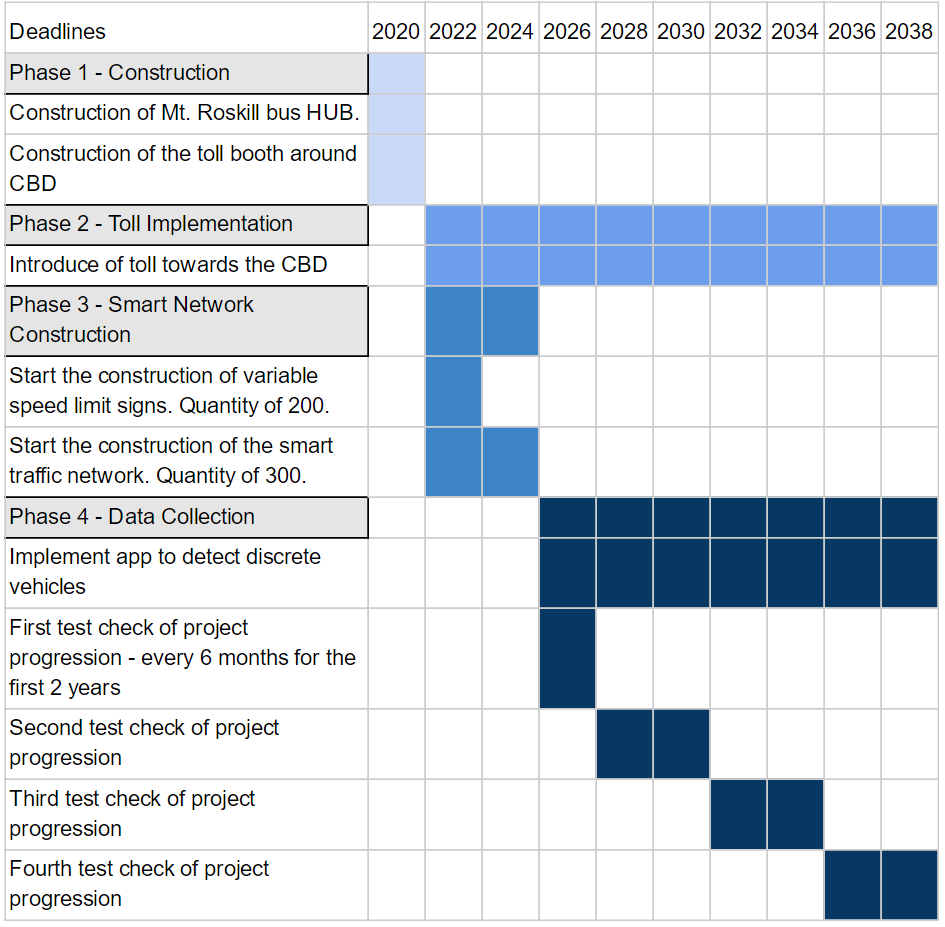
\includegraphics[width=\textwidth]{GANTT.PNG}
\caption{Gantt Chart for the Implementation Plan}
\label{gantt}
\end{table}
\subsection{Cost Estimates}
\begin{table}[H]
\centering
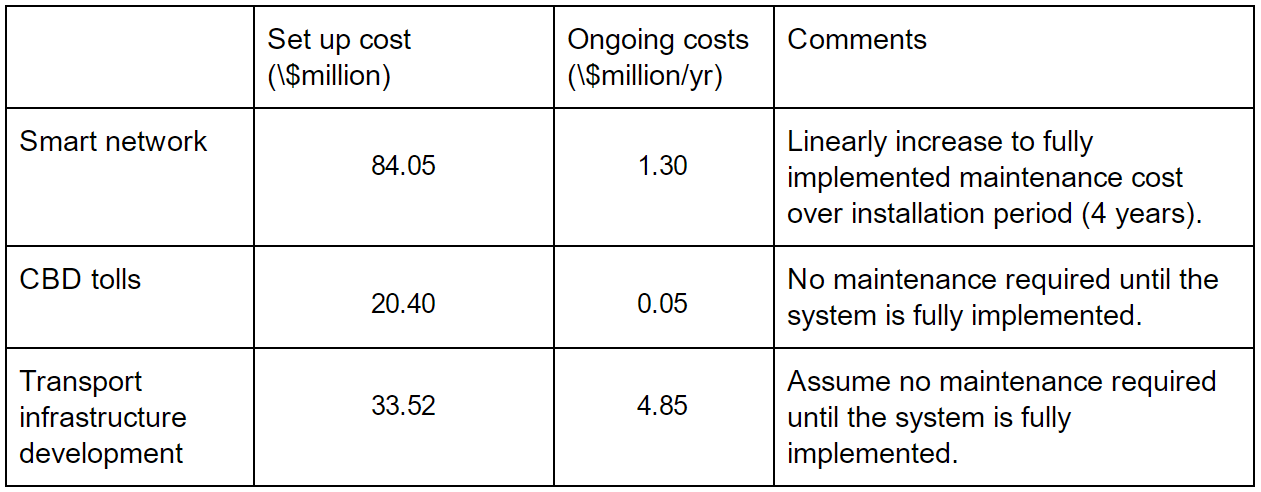
\includegraphics[width=\textwidth]{COSTONE.PNG}
\caption{Cost estimate for the proposed solution}
\label{costone}
\end{table}
\begin{table}[H]
\centering
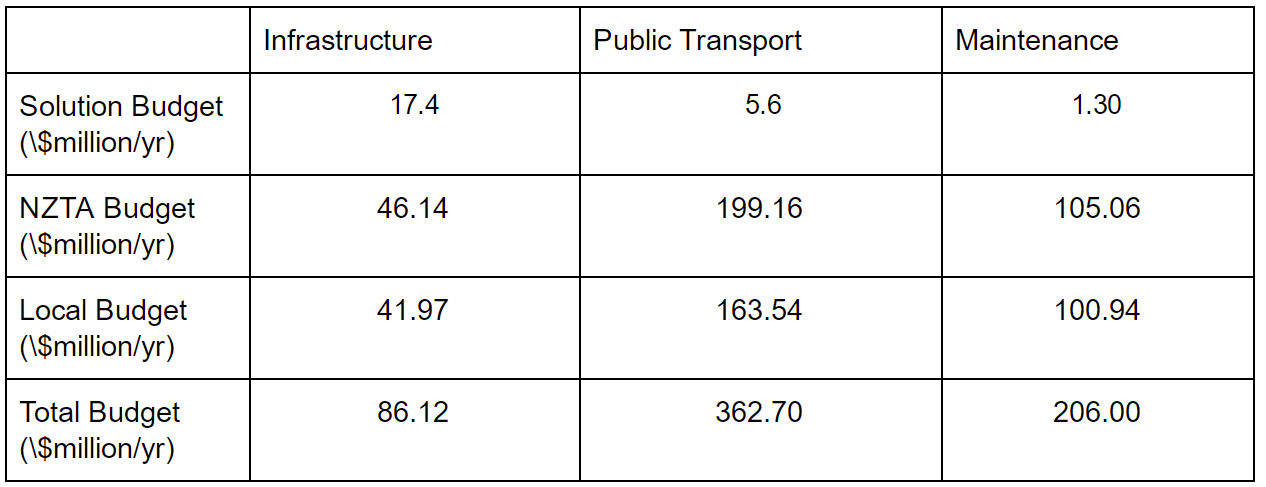
\includegraphics[width=\textwidth]{COSTTWO.PNG}
\caption{Auckland transport cost in comparison to implementation}
\label{costtwo}
\end{table}
The implementation costing is based on a quantitative analysis of all values involved. These values reflect the current estimated costs of material and funding needed on the present day.
\\Transpire accepts that the current value is likely to change due to inflation and may be significantly different before the final investment decision is made. Therefore all value above should be considered estimates and the final cost may vary within 25\%.
\\Costs associated with public announcements, legal matters or future employment have not been accounted for when considering the cost estimate of project implementation. The regional government has been granted the responsibility to determine suitable project process fees needed to internally cover any additional costs they will ensue throughout the implementation of the project.
\\The proposed project has a cost of \$14.2 million dollars for the 6 years of implementation. Implementation budget includes an infrastructure budget allocation of \$52.22 million dollars, a public transport allocation of \$16.76 million and a maintenance allocation of \$1.3 million as the infrastructure NZTA, local and total budgets are \$46.14, \$41.97 and \$86.12 million dollars. As the infrastructure implementation costs are significant in comparison to the total annual infrastructure budget, consideration should be taken into delaying current project plans or reallocation of transport funds throughout regions.
\subsection{Validation}
\subsubsection{Consultation and Analysis Review}
Consultation with stakeholders is undertaken to check if all the requirements are met and let them know the reasoning behind major decisions that were taken. Engineers would receive feedback regarding any issues pointed out by the stakeholders and changes could be made in order to prevent the recurrence of previously made mistakes. An iterative approach would be taken to achieve an efficient final design with maximum benefits. A full analysis of the proposal will be done, with careful refinement along the way. After this, an informed decision would be made to determine the best fit solution.
\subsubsection{Design Review}
All the preliminary designs are reviewed by consulting companies who specialise in tolling systems and smart traffic light networks. The solution is then tested virtually to assess the suitability using software that can model the current CBD traffic. This testing will help us determine the exact locations of the Toll Stations before construction goes ahead and will give us an insight into how the smart traffic lights network will perform.
\subsubsection{Implementation Review}
Extensive testing will be done to maximise efficiency and robustness. Major stakeholders will review the results and point out any issues which need to be resolved. Stakeholders will be updated on regular basis in regards to the construction phase and any difficulties that are being faced. Efforts will be made to resolve any issues pointed out by the stakeholders. These issues could cause a delay in equipment needed to complete the toll stations and Smart Traffic Lights network. 
During the implementation, progress will be checked on a schedule through performance reviews to check the progress of the project on the planned pathway. Since it is difficult to determine the success of the final stage of a 10-year project scope, a time scheme plan with checkpoints of expected outcomes will be used to compare each stage of the implementation into the future.
\subsubsection{Final Review}
After the implementation of the proposed solution, the statistics can be collected in order to validate the reduction in congestion and in travel time. The constant monitoring of the congestion levels after the implementation will give us an idea how much the toll charge should be set to so that people start avoiding driving into the city and make more use of the public transport. After these checks and changes made to toll charge policy, changes will be made to the traffic lights system to optimise the network. The data collected from the toll stations will also be combined with the traffic lights network. The traffic lights network will then have an idea as to how many vehicles are entering the city and from what direction. 
\newpage


\section{Risks and Opportunities}
The implementation of our solution has the capability to generate risks for different divisions such as industry, the public and governing bodies. The risks are characterised by varying probability and impact. If they are both high, they give the most concern. Hence, relevant mitigation plans are crucial to ensure optimum delivery of the project.

\begin{itemize}[leftmargin=0in]
\item Economic Growth \citep{econND}
\begin{enumerate}
\item Reduction in Cost of Production
\begin{enumerate}
\item An efficient transport system will allow for commute time and fuel cost to decrease substantially. This results in the cost of production for a company to decrease and promotes goods and service to have a relatively lower market price.
\end{enumerate}
\item Promotion of Tourism
\begin{enumerate}
\item Our solution provides a faster transportation link between the Auckland Airport and Auckland City, as well as around Auckland. This allows tourists to travel between locations faster and promotes tourist systems. 
\item Faster commutes are aesthetically pleasing for tourist.
\end{enumerate}
\item Increase Production 
\begin{enumerate}
\item The decrease in commute time promotes increasing production. 
\item Workers have more time to be productive, hence jobs/projects completion time decreases. 
\item With the increase in production time of workers companies intake of jobs/projects increases. 
\item Resources will be distributed faster as commute time decreases.
\end{enumerate}
\item Expanding Market
\begin{enumerate}
\item Give commercial businesses to access and expand to new locations in Auckland efficiently.
\end{enumerate}
\item Increase government investment income
\begin{enumerate}
\item Smart Traffic Management starts earning profit after an estimated 2 years. Profit from tolling will help further investment into future transport projects. Smart Traffic Management can allocate its revenue to its maintenance cost.
\end{enumerate}
\end{enumerate}
\item Social Benefit
\begin{enumerate}
\item More employment opportunities:\\By implementing an efficient transport system, this would increase the public's ability to commute to a variety of areas within Auckland. This will increase the number of opportunities where they may seek employment. Also, this would create jobs with respect to transportation of passengers.
\item Increase Health and Well-being:\\To reach their destination on time, travellers have to wake up earlier since they are in traffic for a long duration. With a reduction in sleep and being confined within a vehicle for a long time could cause other health problems such as stress, anxiety and exhaustion for the individual \citep{kylstra14}. With this solution, it will take less time to commute and hence result in a reduction of these side effects promoting good health.
\item The increase in accessibility:\\By constructing bus depots, this will promote accessibility for individuals to public transport. This will give them another incentive to use bus services to avoid the tolling stations in the CBD.  
\item Promoting 'Clean - Green' New Zealand\\New Zealand's 'clean-green' image will be improved by reducing unnecessary greenhouse gas emission due to traffic congestion. This will ultimately provide economical and various benefits to New Zealand.
\item Providing Statistics\\The new implementation will create diverse opportunities for statistical analysis and developing a much deeper understanding of Auckland's traffic flow. The data provided would also be useful for  future project planning and enable more advanced traffic mitigation in New Zealand in the future.
\end{enumerate}
\end{itemize}

\subsection{Smart Network}
\textbf{Economic Risk} - The economic risk associated with the smart network is much greater because of the implementation time and the funds needed for the project. The possibility of completing the project using one year's budget are extremely low. Funds will have to be allocated every year over a period of 4 years. To help in the allocation of funds, the money generated from the electronic tolling can be used. 
\\
\textbf{Social Risk} –  If the app does not catch on and a majority of people don't use it then the smart system will no longer function to its full potential. It is important to make the app appealing and show the benefit of using the app in order for the data collection to be accurate.

\subsection{Electronic Tolling}
\textbf{Economic Risk} - Economic risks associated with Electronic Tolling Project are not significant in the way they can impact the project's completion. The probability of the project failing and not delivering on the assured benefits is extremely low. The BCR ratio shows that the financial value of the benefits will always outweigh the financial cost of implementation or maintenance of this project. To further safeguard this project, a good long term formal contract can be used. The long term contracts will cover various aspects of economic risks associated with the project such as the delays with the construction, increase in the costs of the equipment during the construction, warranties regarding the functioning of the overall toll station. The contract will reduce the share of the risk for the government. Contracts will also help in reducing the `hold-up' behaviour by the companies. Having a good contract will remove uncertainty associated with how the project will be delivered. The Toll will help in generation of funds and therefore will never be a burden for Auckland Transport's budget \citep{dailamietalND}.\\
\textbf{Social Risk} –  Public anger will be present during the project's introduction and implementation. However, with time people will understand the benefits such as fuel costs saving, less congestion and less pollution. The risk is small and will only be present during the early stages of the implementation of the project.
\newpage

\section{Health and Safety}
Construction sites contain heavy machinery and excavated earth which are both significant hazards, therefore, it is our responsibility to ensure the safety of the workers and the general public. All safety checks and NZ standards are to be followed strictly to create a safe working environment and to make sure no fatalities are recorded. Safety concerns have been identified and addressed with considerations for the disabled and elderly.The construction should be done according to the NZS construction guidelines to ensure the durability of the structures and the safety of the vehicles travelling under them during the operation phase.
\begin{itemize}
\item Private vehicles should be restricted from the surrounding area, ensuring smooth flow of buses. Pedestrian crossings must be marked for the disabled and elderly, many of which rely on public transport. 
\item In order to avoid collision of transiting vehicles with the toll booth, ensure there are wide booths accommodating for different car sizes. Careful attention should be paid when deciding on the clearance height of all kinds of vehicles ranging from a motorcycle to a freight truck.
\item Allow for smooth speed transition of cars approaching the toll booths by decreasing the speed limit gradually- likely using the VSLS that are a part of our Smart Network system. Toll signs informing drivers of ticketing prices should be set up a reasonable distance before the booths to make drivers aware of impending toll booth.
\item Queue lines for any possible traffic build up near by toll booth should be clearly outlined on the road.
\item Care is to be taken to ensure the smart algorithms used in the proposed traffic lights works as intended. Traffic lights will still cycle through despite no car detection after an extended period. Traffic monitors will be monitoring the entire system especially during the initial phase for calibration. 
\end{itemize}
\newpage


\section{Expected outcomes}
The brief presented to Transpire Consulting has a broad scope and a variety of ways of defining success - however our best-fit solution provided will effectively combat the growing levels of congestion on Auckland's roads and lead to reduced travel times and increased productivity for residents. The relative level of success of the proposed changes will be proportional to the time that commuting Aucklanders are able to save on their morning/evening trips to and from their respective occupations. Additionally, we have striven to accommodate the needs and requirements of the stakeholders and will use this as another way of measuring the success of the outcomes.
\begin{itemize}
\item Reducing travel times into the CBD during the `rush hour' periods of 6:00am-10am and 3:00-7:00pm was made the priority outcome of our best fit solution, therefore we estimate a significant reduction in time spent in traffic, especially around arterial roads, school zones and areas affected by maintenance construction. This is something that all aforementioned stakeholders will embrace, and will lead to increased support towards Auckland Transport initiatives from all parties moving forward.
\item An economic boost is also expected to be observed as less time spent in traffic leads to increased productivity during the day allowing businesses to maximise their daily turnover. The income that the toll roads will continue to provide into the future will also provide a consistent cash flow stream for mandatory maintenance of existing infrastructure and contribute to other NZTA proposed schemes such as the Auckland Light Rail network.
\item With the expected rise in public transport use comes a proportional drop in cars on the road and fewer cars idling in traffic jams, therefore decreasing greenhouse gas production. This not only benefits the environment as a whole but also reflects fondly on Tourism New Zealand's `clean and green' marketing scheme that we as a country are known around the globe for. If carbon emissions are reduced below New Zealand's emission quota, the carbon credits awarded to the government would be able to further finance carbon reduction schemes between trading partners within New Zealand and around the world.
\item Auckland's population is expected to reach 2 million people by 2033 \citep{stats17} further highlighting the growing housing crisis. The Auckland region will continue to extend further outwards due to the development of new residential areas. With this in mind, our proposed changes have been scaled to develop the transport model in Auckland in a way that will adequately service the inevitable  increase in demand and efficiently account for those residents who are travelling longer distances to get into the CBD.
\item Initially, it can be expected that the inner city tolling will have negative implications on the social standing of NZTA as the general public will see increased day to day costs of travel with little tangible reward. However, with effective communication and marketing to boost public awareness, Transpire Consulting predicts that public opinion toward the proposal will change as they come to terms with the results of their investments. As travel times improve, Auckland residents will benefit from a higher quality of life and standard of living.
\end{itemize}

\newpage


\section{Conclusions and Recommendations}
Auckland City currently has an inadequate solution to its transport issues. Many solutions have been considered to optimise travel in Auckland to minimise travel time and traffic congestion. Transpire Consulting has concluded that the solution proposed by the Government; Smart Traffic Lights, is not sufficient in tackling these issues alone. Transpire Consulting's proposed Smart Traffic Management System; a combination of components, will be implemented to achieve the best solution to address the congestion, travel time and poor driver behaviour found in the city.

The proposed solution is as follows:


\begin{itemize}
\item Electronic Tolling will be placed around the CBD area in an attempt to increase the appeal for public transport. This extra charge should dissuade road users from driving into the city, opting for alternate transport instead. This solution will also provide a source of income that will assist in the funding of the project's other aspects.
\item Smart network and traffic lights will be combined to increase travel efficiency. Using real-time data collected from users, it will improve travel quality by adapting to individual driving behaviour and varying levels of traffic flow at different times of the day. This is used to optimise traffic light intersection operation and create the most efficient travel routes for road users.
\item Lastly a new Transport Hub in Mount Roskill will not only incentivise and increase public transport usage, but also allow for more efficient transport routes. This will help accommodate Auckland's growing population while retaining a future-proof alternative of travel around the city.
\end{itemize}

Auckland City's growth must be factored when considering projects of this scale, therefore it is important that these systems are checked every month. Feedback from a regular check-up schedule will allow for the identification of issues and real-time system optimisation as the city develops into the future.


\newpage
%REFERENCES - Adds to table of contents
\addcontentsline{toc}{section}{List of References}
%REFERENCES - Generates & prints bibliography with title List of References
\printbibliography[title=List of References]


\newpage
%APPENDICES - Starts
\appendix
%APPENDICES - Changes section numbers
\renewcommand{\thesection}{Appendix \Alph{section}}
\renewcommand{\thesubsection}{Appendix \Alph{section}.\arabic{subsection}}


\section{Cost-Benefit Analyses}
\subsection{Smart Traffic Control Network}
We have gathered data from \citep{chan17} on traffic light locations. The number of main road traffic lights in the CBD and Isthmus centre are 185. Allowing for the fact the data is from 2009 and that new traffic lights have been included, we are rounding it up to 200 traffic lights. 

There is currently an existing control centre for traffic management in Auckland (Joint Transport Operations Centre). The improvement proposed improves the data and processing of the information, there is little impact on the control centre. The improvement will provide automated feedback and updates to the traffic system without a controller's input.

Data Collection/Test Checks pertains to the uplink required for each camera to the central processing centre.

Development pertains to the development of a neural net/algorithm to process the input data. An application will also be developed as a companion driver application.

Crash Costs are the costs associated with faster average speeds during commute. As the STCN will improve congestion and reduce commute times, crash costs are to be expected. See \cite[p.~45]{wallis15})

Variable Speed limit signs are signs which go stretch over the highway and display the recommended speed as generated by the central processing centre. 

The maintenance costs are the costs required to maintain and check the cameras and variable speed signs every year. A figure for variable speed signs was not available so an assumption has been made that they have a similar maintenance cost to a billboard and have estimated it as such.

All benefit values were multiplied by a percentage according to their score in the MART analysis table e.g. Schedule delay costs saved was multiplied by 0.7 as it scored 7/10 in terms of its project traffic flow improvement. This was done to account for the fact that no solution will be 100\% effective at reducing congestion. Benefits are calculated from \cite[p.~45]{wallis15}.

Discount rate for infrastructure is 6\% \citep{treasury16}.

The project has been estimated to be complete within four years. Benefits and costs have been calculated using a linear increase. The benefits were calculated by taking the total benefits from the benefits table and placing it as the final figure for year four. As the system gradually upgrades, the benefits will start to be seen and so there is a linear increase from zero to the final \$179.1 million figure. Once year five has been reached, benefits will remain constant as no additional improvement will be added to the STCN.

Cost has been calculated again as a gradual roll out of infrastructure. By end of year four, there needs to be 600 total traffic cameras and 100 variable speed signs. This means there needs to be 150 traffic cameras and 25 variable speed signs installed each year. Maintenance costs then begin the year after. The cost of data collection also linearly increase according to how many cameras have been installed. In Year zero the development costs are added right away. Crash costs are then constant from year one onwards as an improvement in commute speed is to be expected and thus average speed.

\begin{table}[H]
\centering
\resizebox{\textwidth}{!}{%
\begin{tabular}{|l|r|r|r|r|}
\Xhline{2\arrayrulewidth}
\textbf{Based on}&Discount Rate 6\%                                                        & 185 traffic lights &Time to implement: 4 years               &             \\
\Xhline{1\arrayrulewidth}
\textbf{Cost }                                                                    & \textbf{Qty}                &\textbf{ Value (m\$)} &\textbf{Unit Price (m\$)}    &             \\
Camera/Sensor Installation                      & 600               & 30.00 & 0.05 &  \\
Management System                               & 1 - central HUB    & 0.00  &      &  \\
Data Collection/ Test checks                    & 300               & 17.00 & 0.06 &  \\
Development - Neural Net/Algorithm/App upfront) &                   & 0.05  &      &  \\
Crash Costs                    & m\$ p.a & 10.00 &      &  \\
Variable Speed Limit Signs                      & 100               & 27.00 & 0.27 &  \\
Maintenance - Variable Speed Signs              & 100               & 0.50  & 0.01 &  \\
Maintenance - Camera                            & 300               & 0.80  & 0.00 &              \\
\Xhline{1\arrayrulewidth}
\textbf{Benefit}                                            &                    &                &               &             \\
Schedule delay costs saved (traffic flow - 0.7) & m\$ p.a & 69.30  &  &  \\
Travel Time Savings  (traffic flow - 0.7)       &m\$ p.a & 101.50 &  &  \\
Vehicle operating costs saved (economic - 0.7)  & m\$ p.a & 7.70   &  &  \\
Environmental (GHG) Costs saved (enviro - 0.7)  & m\$ p.a & 0.63   &  &  \\
\Xhline{1\arrayrulewidth}
\textbf{Total benefits = sum of benefits}                                         & \textbf{179.13 m\$}             &                &               &             \\
\textbf{Total costs = initial investment - market value + maintenance costs}      & \textbf{85.35 m\$}              &                &               &             \\
assumption: market value = 0 since the solution can't be sold at the end &                    &                &               &             \\
\Xhline{4\arrayrulewidth}
\textbf{Year}& \textbf{Benefit (m\$)} & \textbf{Cost (m\$)}& \textbf{Benefit NPV  (m\$)} & \textbf{Cost NPV (m\$)} \\
0  & 0      & 18.55 & 0      & 18.5 \\
1  & 44.78  & 33.27 & 42.25  & 31.4 \\
2  & 89.57  & 38.05 & 79.71  & 33.9 \\
3  & 134.35 & 42.82 & 112.80 & 36.0 \\
4  & 179.13 & 29.10 & 141.89 & 23.0 \\
5  & 179.13 & 29.10 & 133.86 & 21.7 \\
6  & 179.13 & 29.10 & 126.28 & 20.5 \\
7  & 179.13 & 29.10 & 119.13 & 19.4 \\
8  & 179.13 & 29.10 & 112.39 & 18.3 \\
9  & 179.13 & 29.10 & 106.03 & 17.2 \\
10 & 179.13 & 29.10 & 100.03 & 16.2 \\
11 & 179.13 & 29.10 & 94.36  & 15.3 \\
12 & 179.13 & 29.10 & 89.02  & 14.5 \\
13 & 179.13 & 29.10 & 83.98  & 13.6 \\
14 & 179.13 & 29.10 & 79.23  & 12.9 \\
15 & 179.13 & 29.10 & 74.74  & 12.1 \\
16 & 179.13 & 29.10 & 70.51  & 11.5 \\
17 & 179.13 & 29.10 & 66.52  & 10.8 \\
18 & 179.13 & 29.10 & 62.76  & 10.2 \\
19 & 179.13 & 29.10 & 59.20  & 9.6  \\
20 & 179.13 & 29.10 & 55.85  & 9.1  \\
 &                    & \textbf{Total sum}          & 1811   & 376\\
&                    &                &               &             \\
&                    &                &\cellcolor{green}\textbf{ BCR }          &\cellcolor{green} 4.8\\
\Xhline{2\arrayrulewidth}
\end{tabular}%
}
\caption{Full cost-benefit analysis of the smart traffic control network}
\label{bcastcn}
\end{table}

\newpage
\subsection{Light Rail}
Estimated Installation cost of the Light Rail were based on Table 1, page iii \citep{ATND_3}. We assumed that the rail would be the lower grade. \\

The proposed installation length was based on the map by GreaterAuckland.org \citep{MattL13}. Only the most congested areas were targeted to make this proposal more realistic. 14.4 km of track each way, so 28.8 km, was decided as a reasonable goal to cover these areas.\\

The maintenance and operation costs was based on the 2005 National Transit Database page 62 \citep{nightowler12}. Estimation were made on the assumption that these costs haven't changed.\\

Benefits and Crash Costs have been calculated from \cite[p.~45]{wallis15}.\\

%A - https://at.govt.nz/media/1971157/jmac_report2016-01_emergingtechrapidtransit-part1_apr16.pdf\\

%B - https://www.greaterauckland.org.nz/2017/04/28/cfn2-making-rail-network/\\

%C - http://faculty.washington.edu/kariwat/DE_2005_NTST.pdf

\begin{table}[H]
\centering
\resizebox{\textwidth}{!}{%
\begin{tabular}{|l|r|r|r|r|}
\Xhline{2\arrayrulewidth}
\textbf{Based on}&Discount Rate 6\%&28.8km of Track&Time to implement: 10 years&Light Rail Cars last for about 25 years\\
\Xhline{1\arrayrulewidth}
\textbf{Cost}&\textbf{Qty}&\textbf{Value (m\$)}&\textbf{m\$ per km}&\\
Installation (Length of Network) & 28.8km    & 892.80 & 31.00 &  \\
Operation and maintenance        & per annum & 0.60   & 0.02  &  \\
Crash Costs       & m\$ p.a   & 10     &       &  \\
\Xhline{1\arrayrulewidth}
\textbf{Benefit} &&&&\\
Schedule delay costs saved (traffic flow -1 )  & m\$ p.a & 99    &  &  \\
Travel Time Savings  (traffic flow - 1)        & m\$ p.a & 145   &  &  \\
Vehicle operating costs saved (economic - 0.3) & m\$ p.a & 3.3   &  &  \\
Environmental (GHG) Costs saved (enviro - 8)   & m\$ p.a & 0.72  &  &  \\
Ticket Profit - 25\% of operating costs        & m\$ p.a & 0.149 &  &  \\
\Xhline{1\arrayrulewidth}
\textbf{Total benefits = sum of benefits}                                         & \textbf{248.02 m\$} &  &  &  \\
\textbf{Total costs = initial investment - market value + maintenance costs}      & \textbf{893.40 m\$} &  &  &  \\
assumption: market value = 0 since the solution can't be sold at the end &        &  &  &  \\
\Xhline{4\arrayrulewidth}
\textbf{Year}&\textbf{Benefit (m\$)}&\textbf{Cost (m\$)}&\textbf{Benefit NPV  (m\$)}&\textbf{Cost NPV (m\$)}\\
0  & 0.0   & 89.3  & 0.0   & 89.3  \\
1  & 24.8  & 178.6 & 23.4  & 168.5 \\
2  & 49.6  & 267.8 & 44.1  & 238.4 \\
3  & 74.4  & 357.1 & 62.5  & 299.8 \\
4  & 99.2  & 446.4 & 78.6  & 353.6 \\
5  & 124.0 & 535.7 & 92.7  & 400.3 \\
6  & 148.8 & 625.0 & 104.9 & 440.6 \\
7  & 173.6 & 714.2 & 115.5 & 475.0 \\
8  & 198.4 & 803.5 & 124.5 & 504.1 \\
9  & 223.2 & 892.8 & 132.1 & 528.4 \\
10 & 248.2 & 10.6  & 138.6 & 5.9   \\
11 & 248.2 & 10.3  & 130.7 & 5.4   \\
12 & 248.2 & 10.3  & 123.3 & 5.1   \\
13 & 248.2 & 10.3  & 116.4 & 4.8   \\
14 & 248.2 & 10.3  & 109.8 & 4.6   \\
15 & 248.2 & 10.3  & 103.6 & 4.3   \\
16 & 248.2 & 10.3  & 97.7  & 4.1   \\
17 & 248.2 & 10.3  & 92.2  & 3.8   \\
18 & 248.2 & 10.3  & 86.9  & 3.6   \\
19 & 248.2 & 10.3  & 82.0  & 3.4   \\
20 & 248.2 & 10.3  & 77.4  & 3.2  \\
&&\textbf{Total sum}&  1936.8  &3546.3\\
&&&&\\
&&&\cellcolor{green}\textbf{BCR}&\cellcolor{green}0.55\\
\Xhline{2\arrayrulewidth}
\end{tabular}
}
\caption{Full cost-benefit analysis of the light rail system}
\label{bcalr}
\end{table}
\newpage

\subsection{Electronic Tolls}
Estimated installation costs of electronic tolls systems was found using the total operating expenditure of the Northern gate tolling system seen on page 19 of \citep{ATND_3}. This estimate was based on the assumption the Northern system had four systems installed and with an approximate inflation of toll value of 0.2\%. \\

Estimates toll sensor and camera cost were found on page 14 of \citep{MattL13}. 
Expected revenue for the toll system was estimated with the use of the number of people who travel into the city in peak am time \citep{nightowler12} with the assumption that all people travel alone and that averages are still valid for 2017. We assumed a reduction of 25\% of traffic flow due to tolls and a 90\% charge-ability.\\

Benefits and Crash Costs calculated from \cite[p.~45]{wallis15}.\\

\begin{table}[H]
\centering
\resizebox{\textwidth}{!}{%
\begin{tabular}{|l|r|r|r|r|}
\Xhline{2\arrayrulewidth}
\textbf{Based on}&Discount Rate 6\%&Time to implement: 2 years& &\\
\Xhline{1\arrayrulewidth}
\textbf{Cost}&\textbf{Qty}&\textbf{Value (m\$)}&\textbf{Unit Price (m\$)}&\\
Installation costs        & 17      & 20.4 & 1.2   &  \\
Maintenance costs         & 17      & 0.05 & 0.003 &  \\
Crash costs  & m\$ p.a & 10   &       &  \\
\Xhline{1\arrayrulewidth}
\textbf{Benefit}&&&&\\
Schedule delay costs saved (traffic flow - 0.6) & m\$ p.a & 59.4  &   &  \\
Travel Time Savings  (traffic flow - 0.6)       & m\$ p.a & 87    &   &  \\
Vehicle operating costs saved (economic- 0.8)   & m\$ p.a & 8.8   &   &  \\
Environmental (GHG) Costs saved (enviro - 0.5)  & m\$ p.a & 0.45  &   &  \\
Income earned from tolls                        & m\$ p.a & 39.06 & 5 &  \\
\Xhline{1\arrayrulewidth}
\textbf{Total benefits = sum of benefits}&\textbf{194.7 m\$}&&&\\
\textbf{Total costs = initial investment - market value + maintenance costs}&\textbf{20.4 m\$}&&&\\
\Xhline{4\arrayrulewidth}
\textbf{Year}&\textbf{Benefit (m\$)}&\textbf{Cost (m\$)}&\textbf{Benefit NPV  (m\$)}&\textbf{Cost NPV (m\$)}\\
0  & 0.0   & 20.40 & 0.00   & 20.40 \\
1  & 0.0   & 10.05 & 0.00   & 9.48  \\
2  & 194.7 & 10.05 & 173.29 & 8.94  \\
3  & 194.7 & 10.05 & 163.48 & 8.43  \\
4  & 194.7 & 10.05 & 154.22 & 7.96  \\
5  & 194.7 & 10.05 & 145.50 & 7.51  \\
6  & 194.7 & 10.05 & 137.26 & 7.08  \\
7  & 194.7 & 10.05 & 129.49 & 6.68  \\
8  & 194.7 & 10.05 & 122.16 & 6.30  \\
9  & 194.7 & 10.05 & 115.25 & 5.95  \\
10 & 194.7 & 10.05 & 108.72 & 5.61  \\
11 & 194.7 & 10.05 & 102.57 & 5.29  \\
12 & 194.7 & 10.05 & 96.76  & 4.99  \\
13 & 194.7 & 10.05 & 91.29  & 4.71  \\
14 & 194.7 & 10.05 & 86.12  & 4.44  \\
15 & 194.7 & 10.05 & 81.24  & 4.19  \\
16 & 194.7 & 10.05 & 76.65  & 3.95  \\
17 & 194.7 & 10.05 & 72.31  & 3.73  \\
18 & 194.7 & 10.05 & 68.21  & 3.52  \\
19 & 194.7 & 10.05 & 64.35  & 3.32  \\
20 & 194.7 & 10.05 & 60.71  & 3.13  \\
&&\textbf{Total sum}&  2050  &136\\
&&&&\\
&&&\cellcolor{green}\textbf{BCR}&\cellcolor{green}15\\
\Xhline{2\arrayrulewidth}
\end{tabular}
}
\caption{Full cost-benefit analysis for electronic tolling}
\label{bcaet}
\end{table}
\newpage

\subsection{Developing Public Transport Network}
Construction Costs were gathered from \cite[p.~45]{wallis15} for a length of road.\\

Road maintenance costs were gathered from \cite{MattL13} for the cost to maintain one kilometre of road. We have then estimated the length of road new bus routes from the Mt Roskill hub would cover. We have estimated a direct route to Britomart, then a West East route from New Lynn to Ellerslie.\\

Bus costs and maintenance have been gathered from \cite{nightowler12} per bus. We have then estimated a bus running every 10 minutes which gives us 24 buses we need to cover the routes with the buses.\\

Crash costs are from faster average speeds due to reduced congestion. These costs are from \cite[p.~45]{wallis15})\\

Benefits from reduced congestion from \cite[p.~45]{wallis15}\\

We have also assumed that upfront cost for construction and maintenance costs after completion of the construction. Benefit also increases linearly until completion due to partial operation.\\

\begin{table}[H]
\centering
\resizebox{\textwidth}{!}{%
\begin{tabular}{|l|r|r|r|r|}
\Xhline{2\arrayrulewidth}
\textbf{Based on}&Discount Rate 6\%                                                        &Time to implement: 2 years    &           &             \\
\Xhline{1\arrayrulewidth}
\textbf{Cost}&\textbf{Qty}&\textbf{Value (m\$)}&\textbf{Unit Price (m\$)}&\\
Construction costs & upfront cost & 28.00 &      &  \\
Road maintenance           & 20.8km         & 1.25  & 0.06 &per km  \\
Bus costs                  & 24.0         & 5.52  & 0.23 &  \\
Bus maintenance            & 24.0         & 3.60  & 0.15 &  \\
Crash costs  & m\$ p.a      & 10.00 &      &  \\
\Xhline{1\arrayrulewidth}
\textbf{Benefit}&&&&\\
Schedule delay costs saved (traffic flow - 0.5) & m\$ p.a & 49.50 &  &  \\
Travel Time Savings  (traffic flow - 0.5)       & m\$ p.a & 72.50 &  &  \\
Vehicle operating costs saved (economic- 0.8)   & m\$ p.a & 8.80  &  &  \\
Environmental (GHG) Costs saved (enviro - 0.2)  & m\$ p.a & 0.18  &  &  \\
\Xhline{1\arrayrulewidth}
\textbf{Total benefits = sum of benefits}&\textbf{130.98 m\$}&&&\\
\textbf{Total costs = initial investment - market value + maintenance costs}&\textbf{29.25 m\$}&&&\\
\Xhline{4\arrayrulewidth}
\textbf{Year}&\textbf{Benefit (m\$)}&\textbf{Cost (m\$)}&\textbf{Benefit NPV  (m\$)}&\textbf{Cost NPV (m\$)}\\
0  & 0      & 33.52 & 0     & 33.52 \\
1  & 65.49  & 14.85 & 61.8  & 14.01 \\
2  & 130.98 & 14.85 & 116.6 & 13.22 \\
3  & 130.98 & 14.85 & 110.0 & 12.47 \\
4  & 130.98 & 14.85 & 103.7 & 11.76 \\
5  & 130.98 & 14.85 & 97.9  & 11.10 \\
6  & 130.98 & 14.85 & 92.3  & 10.47 \\
7  & 130.98 & 14.85 & 87.1  & 9.88  \\
8  & 130.98 & 14.85 & 82.2  & 9.32  \\
9  & 130.98 & 14.85 & 77.5  & 8.79  \\
10 & 130.98 & 14.85 & 73.1  & 8.29  \\
11 & 130.98 & 14.85 & 69.0  & 7.82  \\
12 & 130.98 & 14.85 & 65.1  & 7.38  \\
13 & 130.98 & 14.85 & 61.4  & 6.96  \\
14 & 130.98 & 14.85 & 57.9  & 6.57  \\
15 & 130.98 & 14.85 & 54.7  & 6.20  \\
16 & 130.98 & 14.85 & 51.6  & 5.85  \\
17 & 130.98 & 14.85 & 48.6  & 5.51  \\
18 & 130.98 & 14.85 & 45.9  & 5.20  \\
19 & 130.98 & 14.85 & 43.3  & 4.91  \\
20 & 130.98 & 14.85 & 40.8  & 4.63  \\
&&\textbf{Total sum}& 1441   &204\\
&&&&\\
&&&\cellcolor{green}\textbf{BCR}&\cellcolor{green}7.1\\
\Xhline{2\arrayrulewidth}
\end{tabular}
}
\caption{Full cost-benefit analysis of further developing the public transport network}
\label{bcadptn}
\end{table}

\newpage
\section{MART Analysis}
\begin{table}[H]
\centering
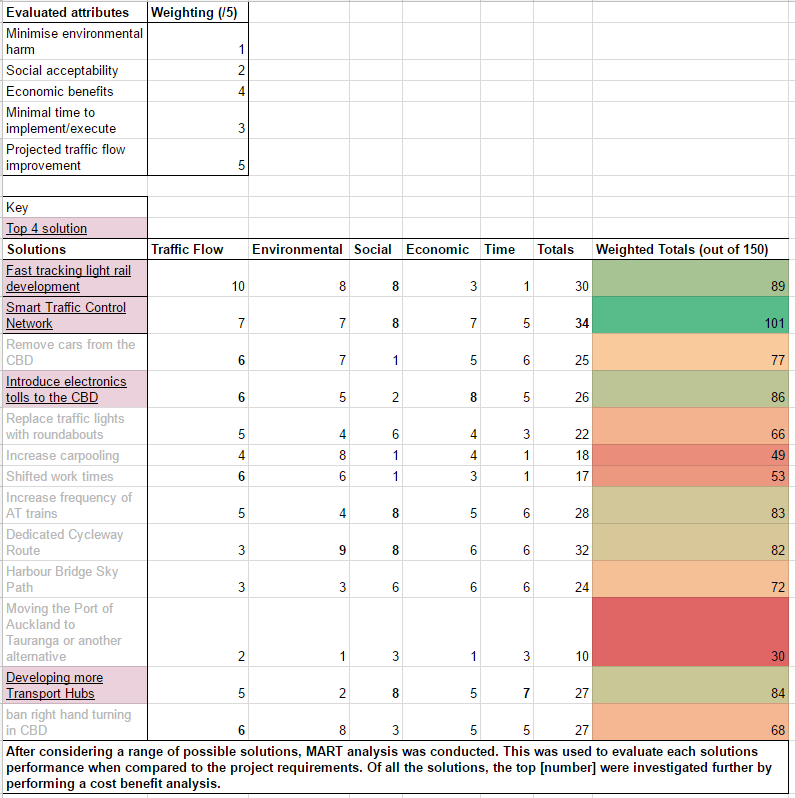
\includegraphics[width=\textwidth]{MART_TABLE_2.PNG}
\caption{MART Analysis}
\label{mart}
\end{table}

\newpage
\section{Toll Road Booth Locations}
\begin{figure}[H]
\centering
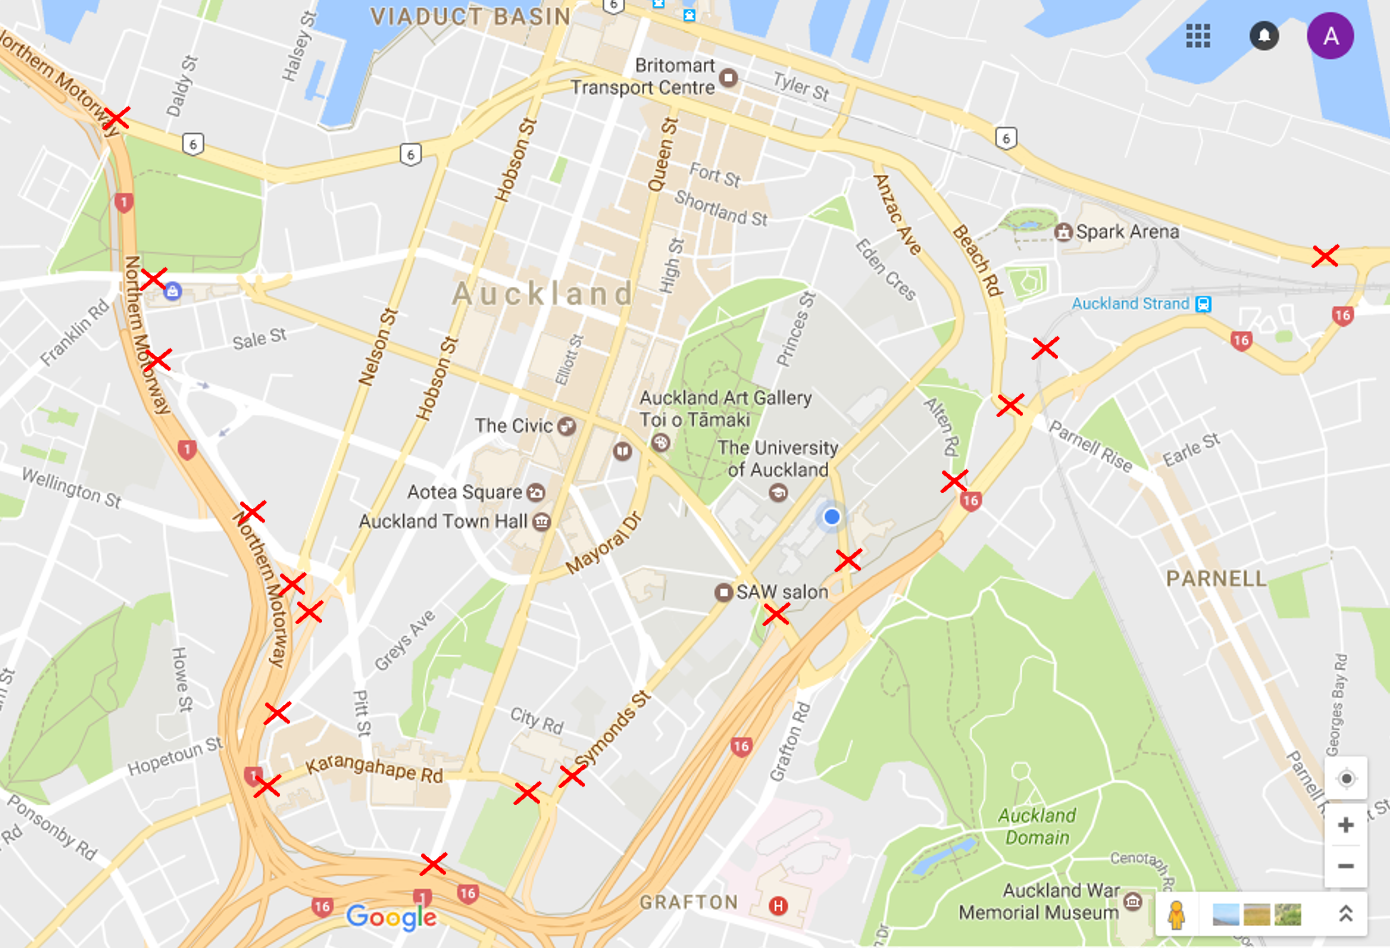
\includegraphics[width=\textwidth]{MAP.png}
\caption{Map of where the toll booths will be located}
\label{fig:tollmap}
\end{figure}

\newpage
\section{Smart Camera Intersection Locations}
\begin{figure}[H]
\centering
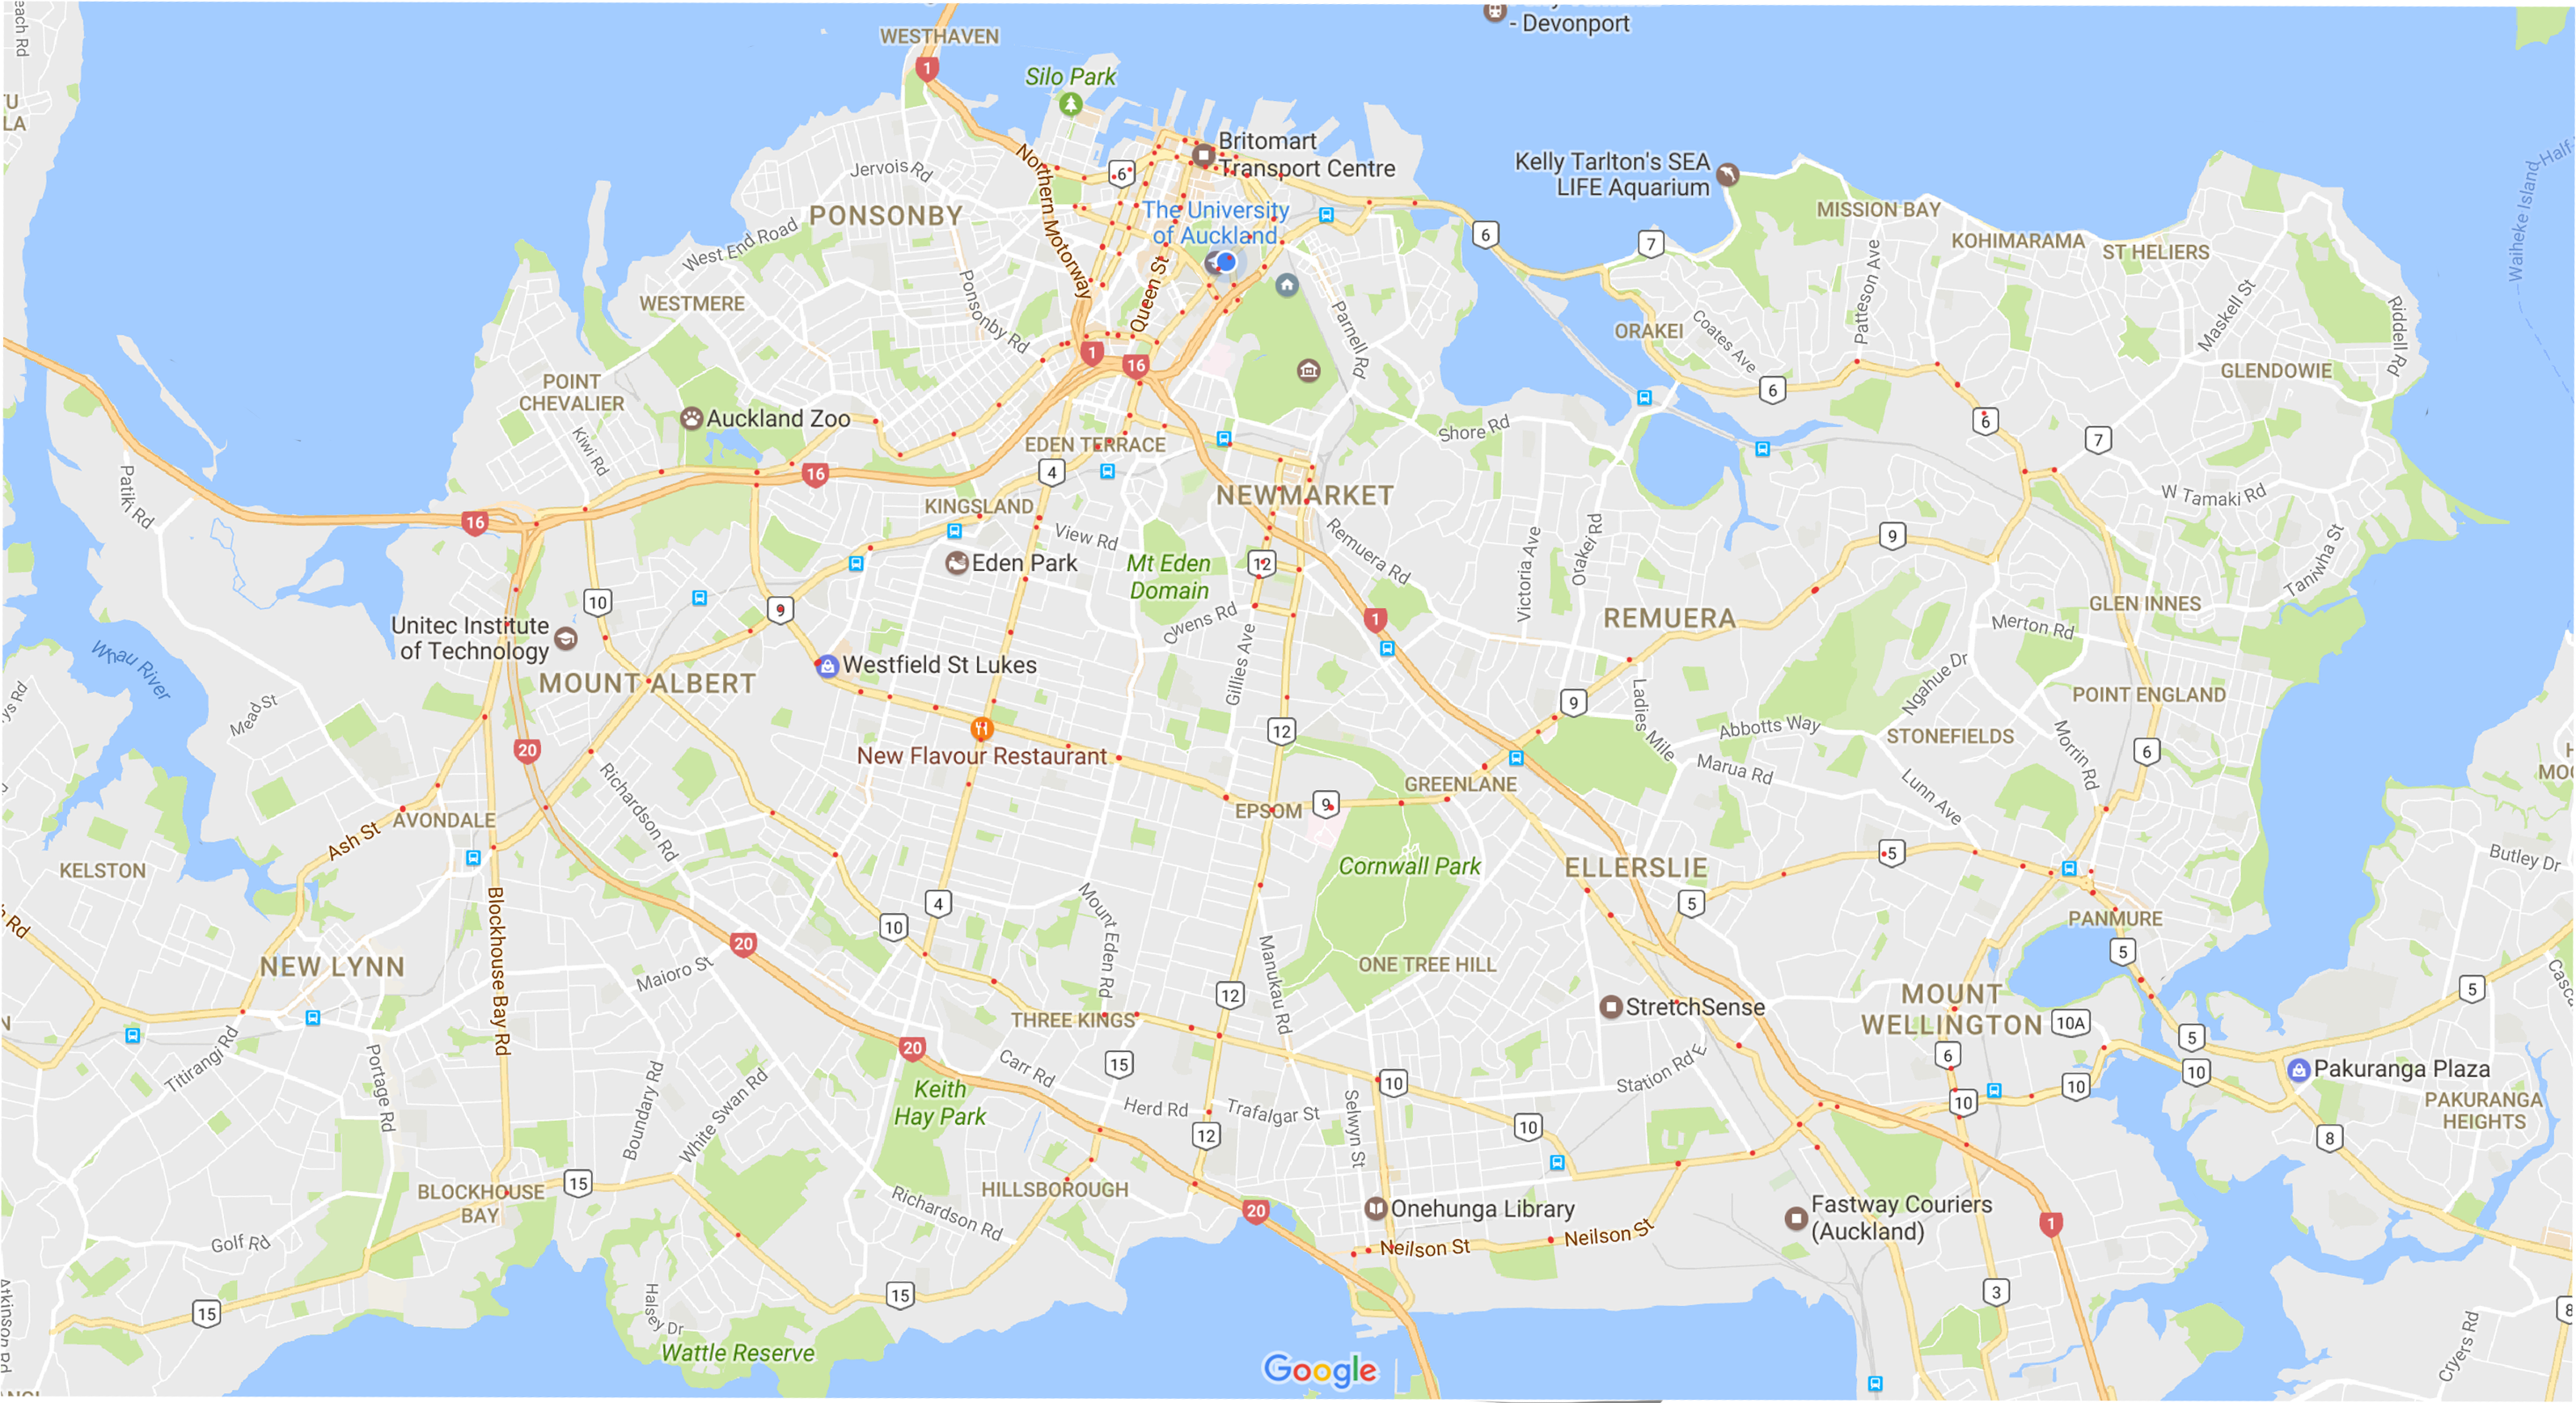
\includegraphics[width=\textwidth]{CAM.png}
\caption{Map of where the smart cameras will be located}
\label{fig:cammap}
\end{figure}
\section{Risks Table}
%table
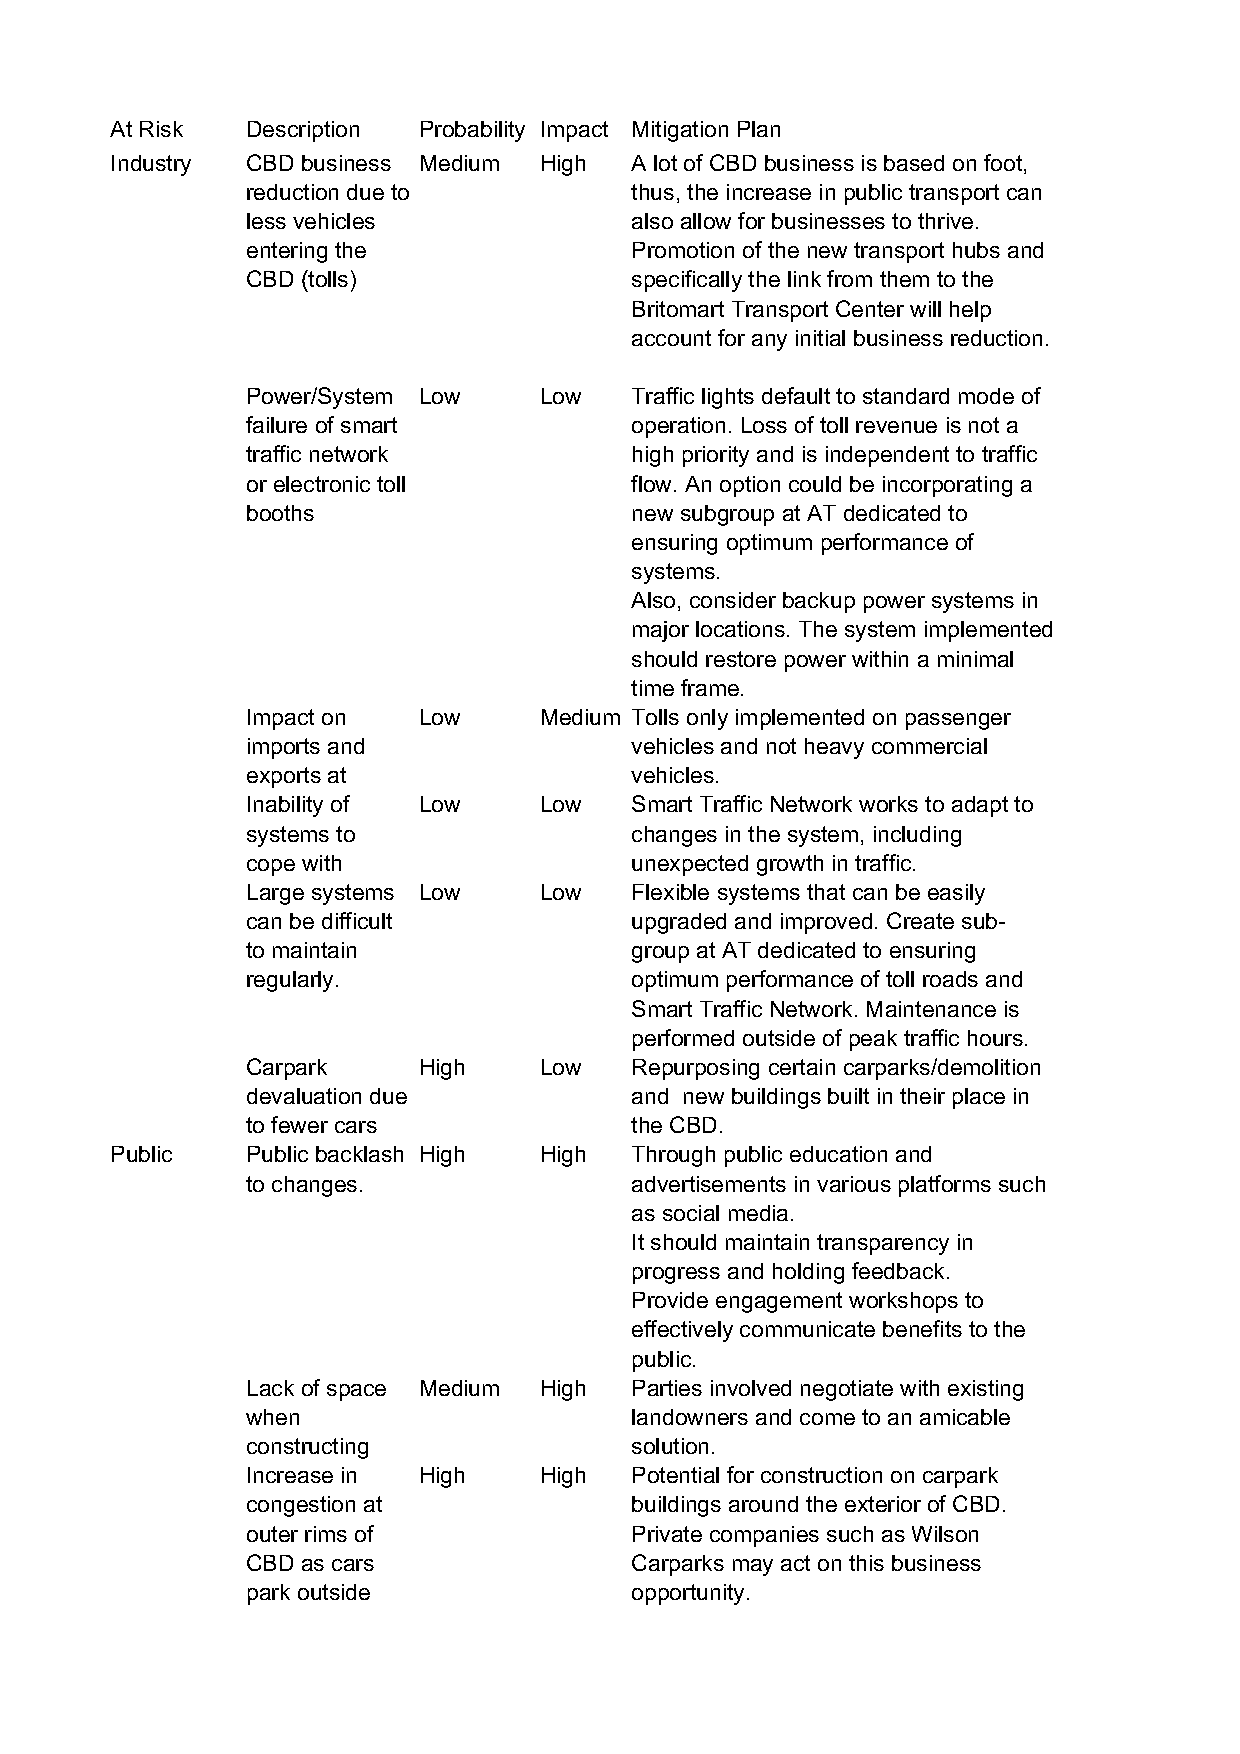
\includepdf[pages=-]{table.pdf}
\label{tab:risks}

%THE END
\end{document}
